\documentclass[12pt,twoside]{mitthesis-exec}

%%%%%%%%%%%%%%%%%%%%%%%%%%%%%%%%%%%%%%%%%%%%%%%%%%%%%%%%%%%%%%%%%%%%%%%%%%%%%%%%
% PREAMBLE

\usepackage[bitstream-charter]{mathdesign} % Use BT Charter font
\usepackage[T1]{fontenc}                   % Use T1 encoding instead of OT1
\usepackage[utf8]{inputenc}                % Use UTF8 input encoding
\usepackage{microtype}                     % Improve typography
\usepackage{amsmath}                       % AMS Math extensions
\usepackage{booktabs}                      % Improve table spacing
\usepackage{graphicx}                      % Extended graphics capabilities
\usepackage{tocbibind}                     % Include listings in TOC
\usepackage[printonlyused]{acronym} % withpage: for showing page of use
\usepackage{listings}                      % Source code listings
\usepackage{caption}
\usepackage{subcaption}
\usepackage[rgb,table]{xcolor}
\usepackage{url}
\usepackage{soul}
\usepackage{array}
\usepackage{pdfpages}
\usepackage{mathtools}
\usepackage{setspace}
\usepackage{pbox}
\usepackage{tikz}
\usetikzlibrary{calc,shapes,decorations.pathreplacing,positioning}
\usepackage{pgfplots}
\usepackage{siunitx}
\usepackage{multirow}
\usepackage{breqn}

% Specialties for tables
\usepackage{array}
\newcolumntype{L}[1]{>{\raggedright\let\newline\\\arraybackslash\hspace{0pt}}m{#1}}
\newcolumntype{C}[1]{>{\centering\let\newline\\\arraybackslash\hspace{0pt}}m{#1}}
\newcolumntype{R}[1]{>{\raggedleft\let\newline\\\arraybackslash\hspace{0pt}}m{#1}}

\usepackage[breaklinks=true]{hyperref}
\hypersetup{colorlinks=true, linkcolor=black, citecolor=black, urlcolor=black,
  pdftitle={Reactor Agnostic Multi-Group Cross Section Generation for Fine Mesh Deterministic Neutron Transport Simulations},
  pdfauthor={William Robert Dawson Boyd}
}
\pagestyle{plain}

%\usepackage{floatrow}
%\floatsetup[table]{style=plaintop}
%\floatsetup[widefigure]{margins=hangleft}

% Highlights and emphasis boxes from Bryans thesis
\usepackage[framemethod=tikz]{mdframed}
\definecolor{mitred}{rgb}{0.698,0.0314,0.216}
\definecolor{mitgray}{rgb}{0.690,0.694,0.710}
\definecolor{canyellow}{rgb}{0.933, 0.965, 0.424}
\newmdenv[nobreak=false, skipabove=2ex, skipbelow=2ex, innerlinewidth=3pt, innerlinecolor=black, backgroundcolor=mitgray!75, roundcorner=10pt, frametitlerule=true, frametitlerulewidth=2.5pt, frametitlefont=\color{white}\Large\bfseries, frametitlealignment=\centering, frametitlebackgroundcolor=mitred, frametitleaboveskip=2ex, frametitlebelowskip=2ex, innertopmargin=3ex, innerbottommargin=2ex]{highlightsbox}
\newmdenv[nobreak=false, skipabove=2ex, skipbelow=2ex, innerlinewidth=2pt, innerlinecolor=black, backgroundcolor=white, roundcorner=10pt]{emphbox}

% Appendix
\usepackage[toc,page]{appendix}

% Don't reset footnote counter between chapters
\usepackage{chngcntr}
\counterwithout{footnote}{chapter}

% Algorithm constructs
\usepackage[chapter]{algorithm} % Provides algorithm environment
\usepackage{algorithmicx}       % Provides algorithmic block
\usepackage{algpseudocode}      % Option of algorithmicx package
\renewcommand{\thealgorithm}{\thechapter-\arabic{algorithm}}
\newcommand\Algphase[1]{%
\vspace*{-.7\baselineskip}\Statex\hspace*{\dimexpr-\algorithmicindent-2pt\relax}\rule{\columnwidth}{0.4pt}%
\Statex\hspace*{-\algorithmicindent}{#1}%
\vspace*{-.7\baselineskip}\Statex\hspace*{\dimexpr-\algorithmicindent-2pt\relax}\rule{\columnwidth}{0.4pt}%
}
\newcommand{\algrule}[1][.4pt]{\par\vskip.5\baselineskip\hrule height #1\par\vskip.5\baselineskip}

% Configure captions
\captionsetup{labelfont=bf, labelsep=colon}
\captionsetup[algorithm]{labelfont=bf, labelsep=colon}

% Use Latin Modern for typewriter fonts
\renewcommand{\ttdefault}{lmtt}

% Add \unit macro
\newcommand{\unit}[1]{\ensuremath{\, \mathrm{#1}}}

\definecolor{gray}{rgb}{0.4,0.4,0.4}
\definecolor{darkblue}{rgb}{0.0,0.0,0.6}
\definecolor{cyan}{rgb}{0.0,0.6,0.6}
\lstset{
  basicstyle=\footnotesize\ttfamily,
  columns=fullflexible,
  showstringspaces=false,
  commentstyle=\color{gray}\upshape,
  frame=single,
  xleftmargin=0.55in
}

\lstdefinelanguage{XML}
{
  morestring=[b]",
  morestring=[s]{>}{<},
  morecomment=[s]{<?}{?>},
  morecomment=[s]{<!--}{-->},
  stringstyle=\color{black},
  identifierstyle=\color{darkblue},
  keywordstyle=\color{cyan},
  morekeywords={}
}

\setcounter{secnumdepth}{4}
\setcounter{tocdepth}{3}

\renewcommand{\contentsname}{Table of Contents}
\renewcommand{\bibname}{References}

\makeatletter \renewcommand\thealgorithm{\arabic{algorithm}} \@addtoreset{algorithm}{chapter} \makeatother

\begin{document}

%%%%%%%%%%%%%%%%%%%%%%%%%%%%%%%%%%%%%%%%%%%%%%%%%%%%%%%%%%%%%%%%%%%%%%%%%%%%%%%%
% TITLE PAGE

\title{EXECUTIVE SUMMARY \\~\\ Reactor Agnostic Multi-Group Cross Section Generation for Fine Mesh Deterministic Neutron Transport Simulations}

\author{William Robert Dawson Boyd III}
\prevdegrees{B.S., Georgia Institute of Technology (2010) \\
             M.S., Massachusetts Institute of Technology (2014)}
\department{Department of Nuclear Science and Engineering}
\degree{Doctor of Philosophy in Nuclear Science and Engineering}

\degreemonth{February}
\degreeyear{2017}
\thesisdate{November 4, 2016}

\supervisor{Benoit Forget}{Associate Professor of Nuclear Science and Engineering}
\reader{Kord S. Smith}{KEPCO Professor of the Practice of Nuclear Science and Engineering}
\chairman{Emilio Bagglietto}{Associate Professor of Nuclear Science and Engineering}


%%%%%%%%%%%%%%%%%%%%%%%%%%%%%%%%%%%%%%%%%%%%%%%%%%%%%%%%%%%%%%%%%%%%%%%%%%%%%%%%
%%%%%%%%%%%%%%%%%%%%%%%%%%%%%%%%%%%%%%%%%%%%%%%%%%%%%%%%%%%%%%%%%%%%%%%%%%%%%%%%
% ABSTRACT

\setcounter{savepage}{\thepage}

\begin{abstractpage}

The development of high fidelity multi-group neutron transport-based simulation tools for full core Light Water Reactor (LWR) analysis has been a long-standing goal of the reactor physics community. While direct transport simulations have previously been far too computationally expensive, advances in computer hardware have allowed large scale simulations to become feasible. Therefore, many have focused on developing full core neutron transport solvers that do not incorporate the approximations and assumptions of traditional nodal diffusion solvers. 

Due to the computational expense of direct full core 3D deterministic neutron transport methods, many have focused on 2D/1D methods which solve 3D problems as a coupled system of radial and axial transport problems. However, the coupling of radial and axial problems also introduces approximations. Instead, the work in this thesis focuses on explicitly solving the 3D deterministic neutron transport equations with the Method of Characteristics (MOC).

MOC has been widely used for 2D lattice physics calculations due to its ability to accurately and efficiently simulate reactor physics problems with explicit geometric detail. The work in this thesis strives to overcome the significant computational cost of solving the 3D MOC equations by implementing efficient track generation, axially extruded ray tracing, Coarse Mesh Finite Difference (CMFD) acceleration, linear track-based source approximations, and scalable domain decomposition. 

Additionally, significant attention has been be given to complications that arise in full core simulations with transport-corrected cross-sections. The convergence behavior of transport methods is analyzed, leading to a new strategy for stabilizing the source iteration scheme for neutron transport simulations. The methods are incorporated into the OpenMOC reactor physics code and simulation results are presented for the full core BEAVRS LWR benchmark. Parameter refinement studies and comparisons with reference OpenMC Monte Carlo solutions show that converged full core 3D MOC simulations are feasible on modern supercomputers for the first time.

%However, 3D full core LWR simulations present significant challenges due to greatly increased computational cost.

%The Method of Characteristics (MOC) has seen wide interest in reactor physics because of its accuracy and efficiency in computing lattice physics problems. While most of its use has been in solving 2D problems, there has been recent interest in extending MOC to 3D in order to more accurately calculate 3D power distributions in LWRs. While the method is naturally extensible to 3D, it presents significant computational difficulties. Methods will be presented which mitigate the computational difficulties of 3D MOC by using domain decomposition, efficient track generation, axially extruded ray tracing, CMFD acceleration, and a linear source approximation. Significant attention will be given to complications that arise in full core simulations. 3D MOC results will be presented for the full core simulation of the BEAVRS benchmark, showing that 3D MOC can be a viable tool for anal

\end{abstractpage}

\singlespacing 

%%%%%%%%%%%%%%%%%%%%%%%%%%%%%%%%%%%%%%%%%%%%%%%%%%%%%%%%%%%%%%%%%%%%%%%%%%%%%%%%
\section*{Introduction}

%%%%%%%%%%%%%%%%%%%%%%%%%%%%%%%%%%%%%%%
\subsection*{Background and Motivation}

-brief literature review\\
  -use MC to generate coarse mesh constants (Serpent)~\cite{serpent2013manual} \\
  -relatively little work to use MC for fine mesh transport~\cite{redmond1997multigroup,cai2014condensation,nelson2014improved} \\

\begin{emphbox}
\textbf{This thesis is motivated by the desire to obtain Monte Carlo-quality solutions with computationally efficient deterministic neutron transport methods.}
\end{emphbox}

\begin{figure}[h!]
\centering
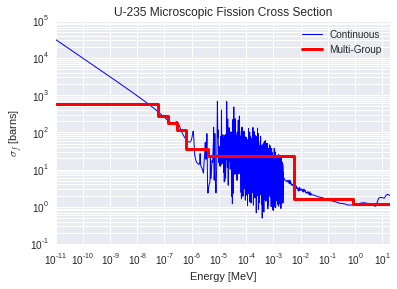
\includegraphics[width=0.6\linewidth]{figures/intro/u235-ce-mg-xs}
\caption[U-235 continuous energy and multi-group fission cross section]{U-235 continuous energy and 16-group fission cross section.}
\label{fig:u235-sigf}
\end{figure}

\begin{figure}[h!]
\centering
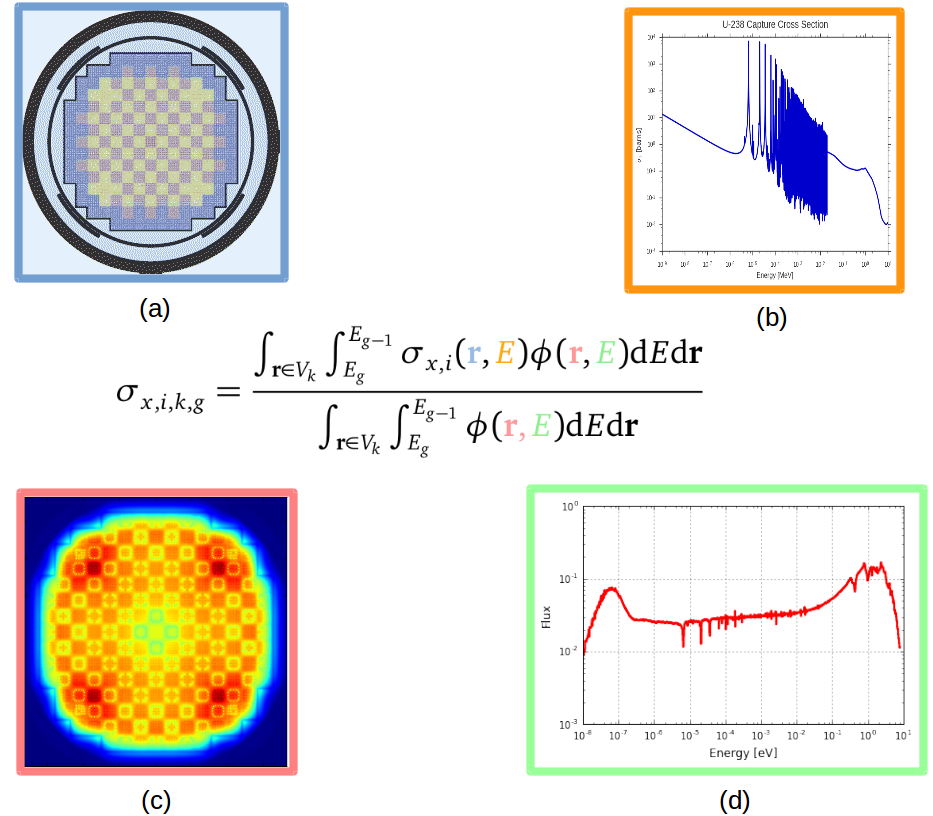
\includegraphics[width=0.9\linewidth]{figures/mgxs/mgxs-overlay}
\caption[Energy and spatial variation in MGXS]{The calculation of multi-group cross sections requires knowledge of the spatial and energy variation of the continuous energy cross section and flux. The color-coded position $\mathbf{r}$ and energy $E$ variables correspond to the figures with the matching colored outlines. The microscopic cross section $\sigma_{x,i}$ depends on reactor configuration (a) and neutron energy (b). The flux $\phi$ varies with position (c) and energy (d).}
\label{fig:mgxs-overlay}
\end{figure}

\begin{figure}[h!]
\centering
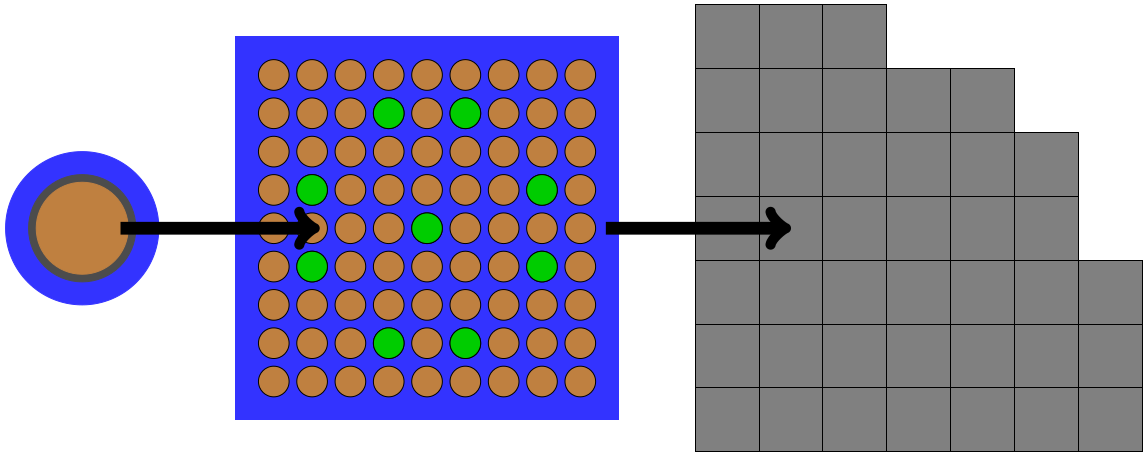
\includegraphics[width=0.9\linewidth]{figures/intro/multi-step-flow-chart}
\caption[Multi-level approach to reactor analysis]{Current multi-level framework for reactor analysis.}
\label{fig:multi-level-flow-chart}
\end{figure}

\begin{emphbox}
\textbf{This thesis develops and evaluates MC-based methods to generate MGXS for fine mesh deterministic neutron transport codes.}
\end{emphbox}

\begin{emphbox}
\textbf{This thesis uses statistical clustering algorithms to accelerate whole-core MC calculations
which simultaneously model all energy and spatial self-shielding effects for fine mesh MGXS generation in a single step.}
\end{emphbox}

\clearpage

%%%%%%%%%%%%%%%%%%%%%%%%
\subsection*{Objectives}

The subject matter of this thesis is organized along two main themes:

\begin{itemize}
\item \textbf{\textit{Approximation Error}} -- Quantify and diagnose approximation error in MGXS generated from MC methods for simple heterogeneous benchmark problems.
\item \textbf{\textit{Statistical Clustering}} -- Develop statistical clustering methods to accelerate the convergence of MGXS on heterogeneous MC tally meshes.
\end{itemize}

\clearpage

%%%%%%%%%%%%%%%%%%%%%%%%%%%%%%%%%%%%%%%%%%%%%%%%%%%%%%%%%%%%%%%%%%%%%%%%%%%%%%%%
\section*{Software Infrastructure: A Simulation Triad}

-OpenMC~\cite{romano2013openmc} generates MGXS \\
-OpenMOC~\cite{boyd2014openmoc} uses MGXS in deterministic multi-group transport calculations \\
-OpenCG~\cite{boyd2015opencg} enables processing and transfer of tally data  \\

\begin{figure}[h!]
  \centering
  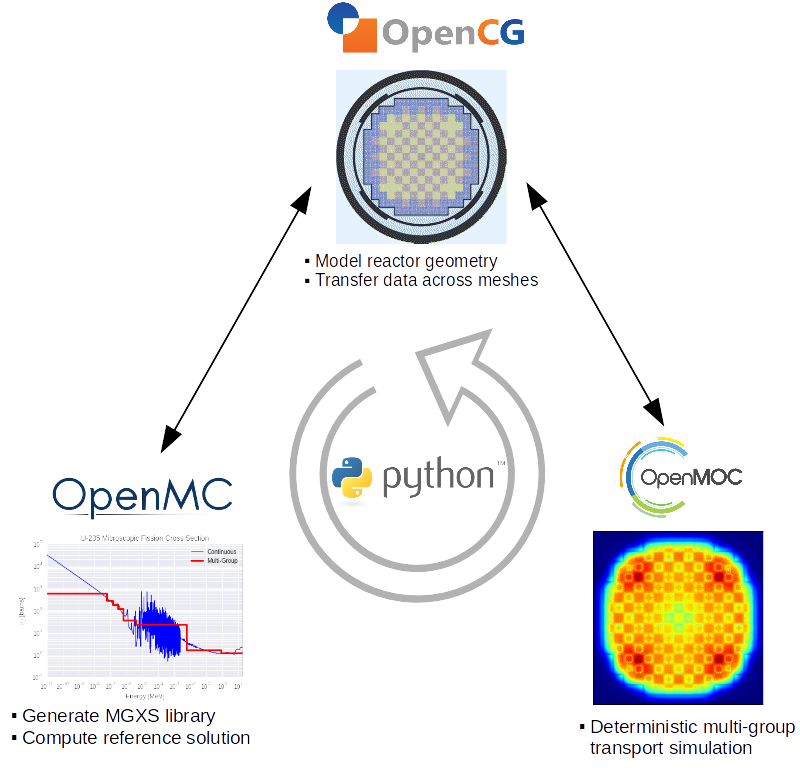
\includegraphics[width=\linewidth]{figures/workflow/triad/simulation-triad}
\caption[A simulation triad of OpenMC, OpenMOC and OpenCG]{A simulation triad consisting of the OpenMC, OpenMOC and OpenCG codes ``glued'' together with Python formed the foundation for this thesis research.}
\label{fig:simulation-triad}
\end{figure}

\clearpage

%%%%%%%%%%%%%%%%%%%%%%%%%%%%%%%%%%%%%%%%%%%%%%%%%%%%%%%%%%%%%%%%%%%%%%%%%%%%%%%%
\section*{Angular-Dependent MGXS and SPH Factors}

%%%%%%%%%%%%%%%%%%%%%%%%%%%%%%%%%%%%%%%%%%%%%
\subsection*{Flux Separability Approximation}

\begin{dmath}
\label{eqn:sigt-flux-separable}
\Sigma_{t,g}(\mathbf{r}) = \frac{\int\displaylimits_{E_{g}}^{E_{g-1}} \Sigma_{t}(\mathbf{r},E)\psi(\mathbf{r},\mathbf{\Omega},\mathrm{d}E)}{\psi_{g}(\mathbf{r},\mathbf{\Omega})} \approx \frac{\int\displaylimits_{E_{g}}^{E_{g-1}} \Sigma_{t}(\mathbf{r},E)\phi(\mathbf{r},E)}{\phi_{g}(\mathbf{r})}
\end{dmath}

\clearpage

%%%%%%%%%%%%%%%%%%%%%%%%%%%%%%%%%%%%%%%%%%
\subsection*{Energy-Dependent Flux Errors}

\begin{figure}[h!]
\centering
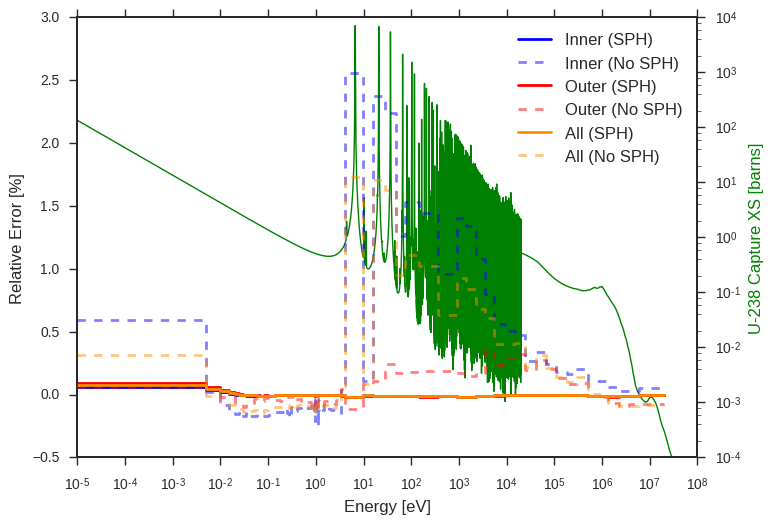
\includegraphics[width=\linewidth]{figures/sph/pin-cell/rel-err-inner-outer}
\caption[Flux relative error by energy group with SPH]{The energy-dependent relative error of the 70-group OpenMOC scalar flux with respect to the OpenMC flux in a fuel pin for the innermost, outermost and all FSRs.}
\label{fig:rel-err-energy}
\end{figure}

\clearpage

%%%%%%%%%%%%%%%%%%%%%%%%%%%%%%%%%%%%
\subsection*{Angular-Dependent MGXS}

\begin{figure}[h]
\begin{subfigure}{.5\textwidth}
  \centering
  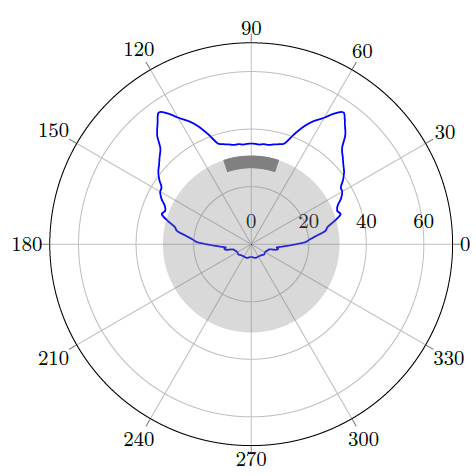
\includegraphics[width=\linewidth]{figures/sph/batman-1}
  \caption{}
  \label{fig:batman-plots-a}
\end{subfigure}
\begin{subfigure}{.5\textwidth}
  \centering
  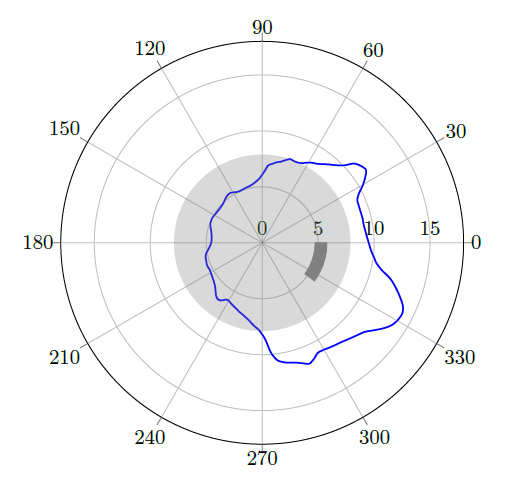
\includegraphics[width=\linewidth]{figures/sph/batman-2}
  \caption{}
  \label{fig:batman-plots-b}
\end{subfigure}
\caption[Angular-dependent capture MGXS]{Angular-dependent capture MGXS for the 6.67 eV resonance group as a function of azimuthal angle for two different FSRs. The radial axis is given in units of barns and the azimuthal axis in units of degrees. \textit{Image courtesy of N. Gibson~\cite{gibson2016thesis}.}}
\label{fig:batman-plots}
\end{figure}

\clearpage

%%%%%%%%%%%%%%%%%%%%%%%%%%%%%%%%%%%%%%%%%%%%%%%%%%
\subsection*{SuPerHomog\'{e}n\'{e}isation Factors}

-SPH factors were first proposed by H\'{e}bert~\cite{hebert1993consistent} to preserve reaction rates during energy condensation and spatial homogenization \\
-SPH factor algorithm requires knowledge of a reference source that is used in a multi-group fixed source solver to derive multiplicative factors that adjust the total MGXS to force neutron balance \\

\begin{dmath}
\label{eqn:sph-transport-eqn-iterate}
\mathbf{\Omega} \cdot \nabla \psi_{g}^{(n)}(\mathbf{r},\mathbf{\Omega}) + \mu_{k,g}^{(n-1)}\Sigma_{t,k,g}\psi_{g}^{(n)}(\mathbf{r},\mathbf{\Omega}) = Q_{k,g}(\mathbf{\Omega})
\end{dmath}

\begin{dmath}
\label{eqn:sph-update-sigt}
\Sigma_{t,k,g}^{(n)} = \mu_{k,g}^{(n-1)}\Sigma_{t,k,g}^{(0)}
\end{dmath}

\begin{algorithm}[h]
\caption{SPH Factor Algorithm}
\label{alg:sph}
\begin{algorithmic}[1]
%  \State Initialize MGXS from MC tallies
%  \State Compute neutron source from MC flux and MGXS
  \State Initialize SPH factors to unity
  \While{SPH factors are not converged}
    \State Update MGXS with SPH factors \Comment{Eqn.~\ref{eqn:sph-update-sigt}}
    \State Solve fixed source transport problem \Comment{Eqn.~\ref{eqn:sph-transport-eqn-iterate}}
    \State Compute new SPH factors
  \EndWhile
  \State Compute final MGXS with SPH factors \Comment{Eqn.~\ref{eqn:sph-update-sigt}}
\end{algorithmic}
\end{algorithm}

\begin{table}[h!]
  \centering
  \caption[Eigenvalues with and without SPH factors for a fuel pin]{The impact of SPH factors on the eigenvalue bias $\Delta\rho$ with varying energy group structures for a fuel pin.}  
  \label{table:sph-keff}
  \vspace{6pt}
  \begin{tabular}{c S[table-format=6.1] S[table-format=6.1]}
  \toprule
  & \multicolumn{2}{c}{{\bf $\boldsymbol{\Delta\rho}$ [pcm]}} \\
  \cline{2-3}
  \multirow{-2}{*}{{\bf \# Groups}} &
  \multicolumn{1}{c}{{\bf Without SPH}} &
  \multicolumn{1}{c}{{\bf With SPH}} \\
  \midrule
1 & 66 & -14 \\
2 & 34 & -6\\
4 & -57 & 1 \\
8 & -102 & 2 \\
16 & -111 & 4 \\
25 & -182 & -1 \\
40 & -202 & 2 \\
70 & -211 & -3 \\
  \bottomrule
\end{tabular}
\end{table}

\clearpage

%%%%%%%%%%%%%%%%%%%%%%%%%%%%%%%%%%%%%%%%%
\section*{Spatial Homogenization Schemes}

%%%%%%%%%%%%%%%%%%%%%%%%%%%%%%%%%%%%%%%%%%%%%%%%%%%
\subsection*{Track Density-Weighted Homogenization}

\begin{equation}
\label{eqn:imgxs-set}
\mathbb{S}_{m} = \left\{1 \le k \le K: S(k) = m\right\}
\end{equation}

LNS homogenization computes a single set of MGXS for the fuel pin instances in each set $k \in \mathbb{S}_{m}$ classified by the LNS algorithm. This is equivalent to a specialization of Eqn.~\ref{eqn:imgxs-micro} with track density-weighted averages of the reaction rates and flux tallies in each pin instance:

\begin{equation}
\label{eqn:imgxs-micro}
\hat{\sigma}_{x,i,m,g} = \frac{\displaystyle\sum\limits_{k=1}^{K}\mathbb{1}_{\mathbb{S}_{m}}(k) \langle \sigma_{x,i}, \psi \rangle_{k,g}^{t\ell}}{\displaystyle\sum\limits_{k=1}^{K}\mathbb{1}_{\mathbb{S}_{m}}(k) \langle \psi \rangle_{k,g}^{t\ell}}
\end{equation}

%%%%%%%%%%%%%%%%%%%%%%%%%%%%%%%%%
\subsection*{Null Homogenization}

%%%%%%%%%%%%%%%%%%%%%%%%%%%%%%%%%%%%%%%
\subsection*{Degenerate Homogenization}

%%%%%%%%%%%%%%%%%%%%%%%%%%%%%%%%
\subsection*{LNS Homogenization}

%%%%%%%%%%%%%%%%%%%%%%%%%%%%%%%%%%%%%%%%%%%
\subsection*{\textit{i}MGXS Homogenization}

\begin{figure}[h!]
\centering
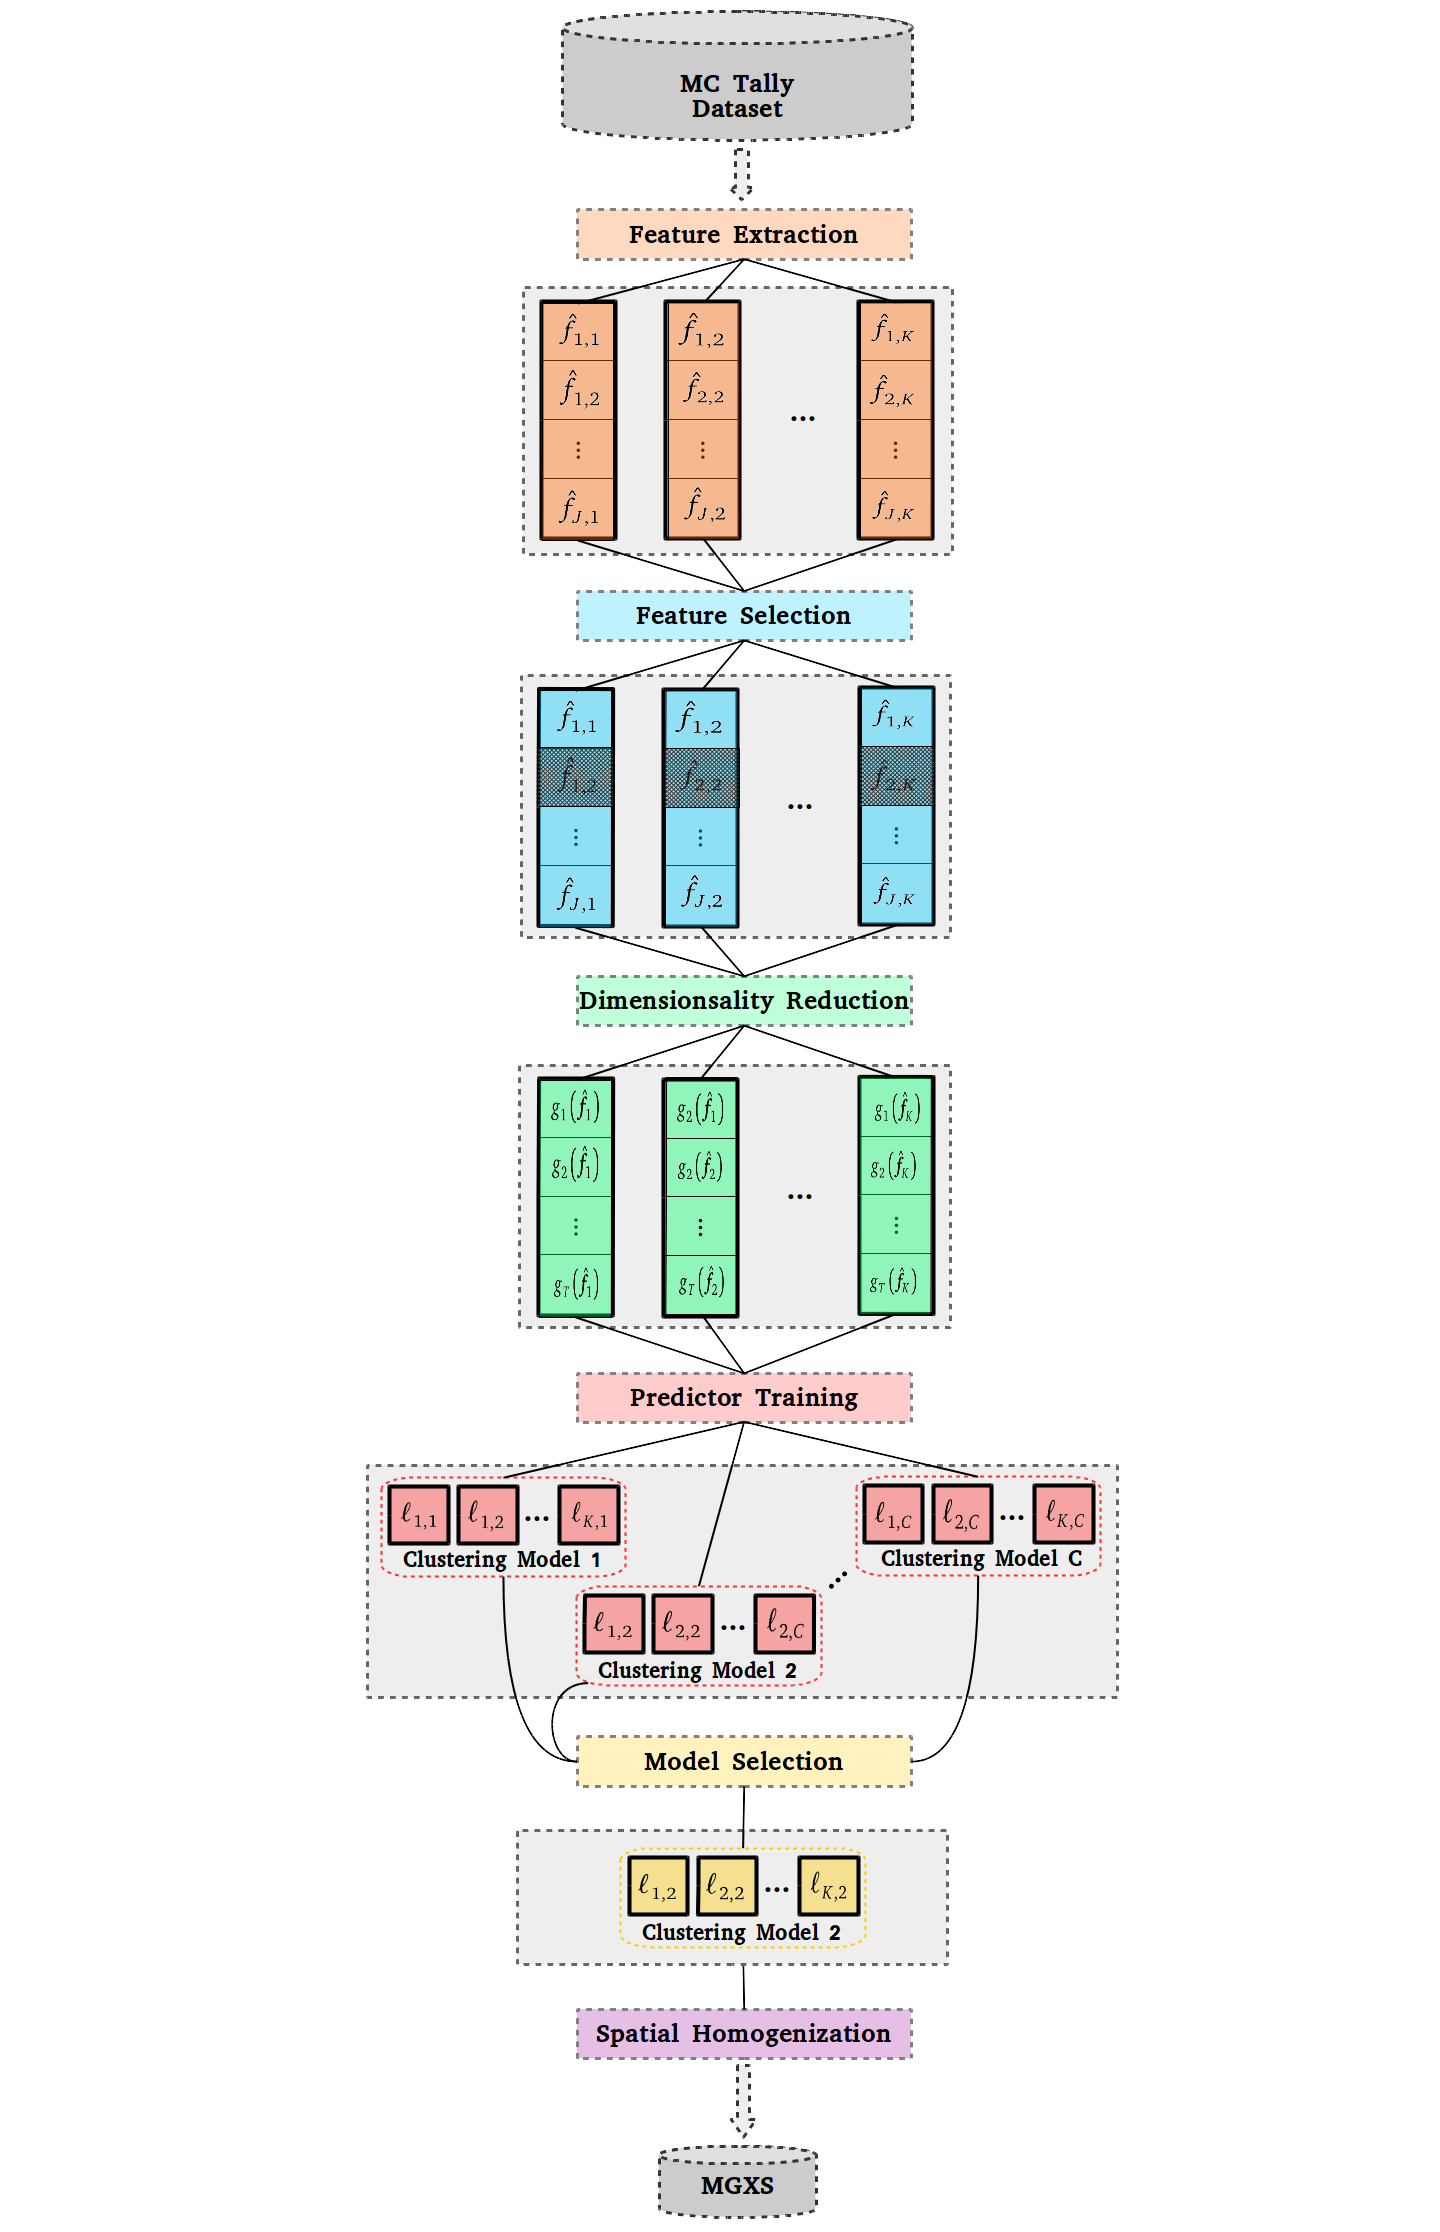
\includegraphics[width=0.9\linewidth]{figures/unsupervised/features/engineering/flow-chart}
\vspace{2mm}
\caption[\textit{i}MGXS flow chart]{The \textit{i}MGXS data processing pipeline.}
\label{fig:imgxs-flow-chart}
\end{figure}

\begin{figure}[h!]
\centering
\begin{subfigure}{0.45\textwidth}
  \centering
  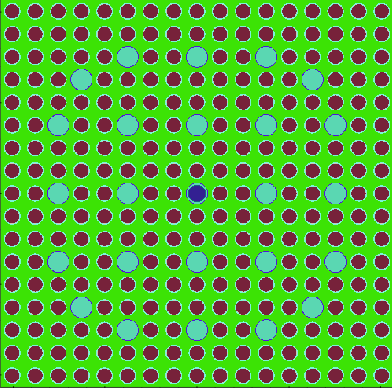
\includegraphics[width=0.9\linewidth]{figures/unsupervised/features/assm-16/geometry}
  \caption{}
  \label{fig:capt-mean-std-geom}
\end{subfigure}%
\begin{subfigure}{0.45\textwidth}
  \centering
  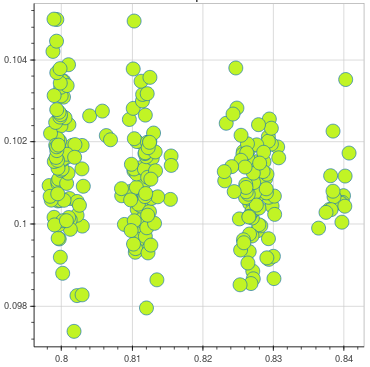
\includegraphics[width=0.9\linewidth]{figures/unsupervised/features/assm-16/u238-capt/mean-std/mgxs}
  \caption{}
  \label{fig:capt-mean-std-mgxs}
\end{subfigure}
\begin{subfigure}{0.45\textwidth}
  \centering
  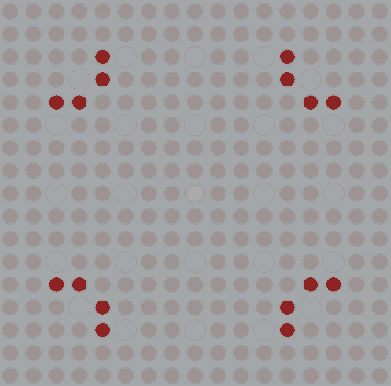
\includegraphics[width=0.9\linewidth]{figures/unsupervised/features/assm-16/u238-capt/mean-std/geometry-3}
  \caption{}
  \label{fig:capt-mean-std-geom-3}
\end{subfigure}%
\begin{subfigure}{0.45\textwidth}
  \centering
  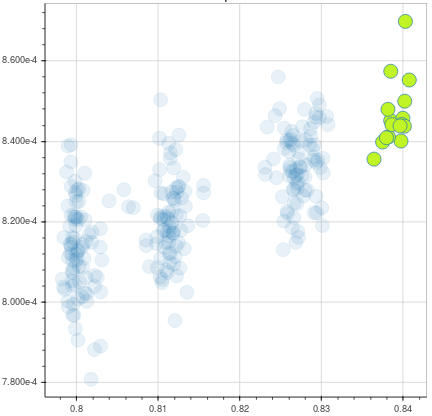
\includegraphics[width=0.9\linewidth]{figures/unsupervised/features/assm-16/u238-capt/mean-std/mgxs-3}
  \caption{}
  \label{fig:capt-mean-std-mgxs-3}
\end{subfigure}
\caption[Clustering of U-238 capture MGXS standard deviations]{Scatter plots of the pin-wise U-238 capture (group 1 of 2) MGXS means ($x$) and standard deviations ($y$) for a 1.6\% enriched fuel assembly.}
\label{fig:capt-mean-std}
\end{figure}

\clearpage

%%%%%%%%%%%%%%%%%%%%%%%%%%%
\section*{Model Validation}

%%%%%%%%%%%%%%%%%%%%%%%%%%%%%%%%%%%%%%%%%%
\subsection*{Heterogeneous PWR Benchmarks}

-construction of six heterogeneous benchmarks from BEAVRS~\cite{horelik2013beavrs} \\

\begin{figure}[h!]
\centering
\begin{subfigure}{0.47\textwidth}
  \centering
  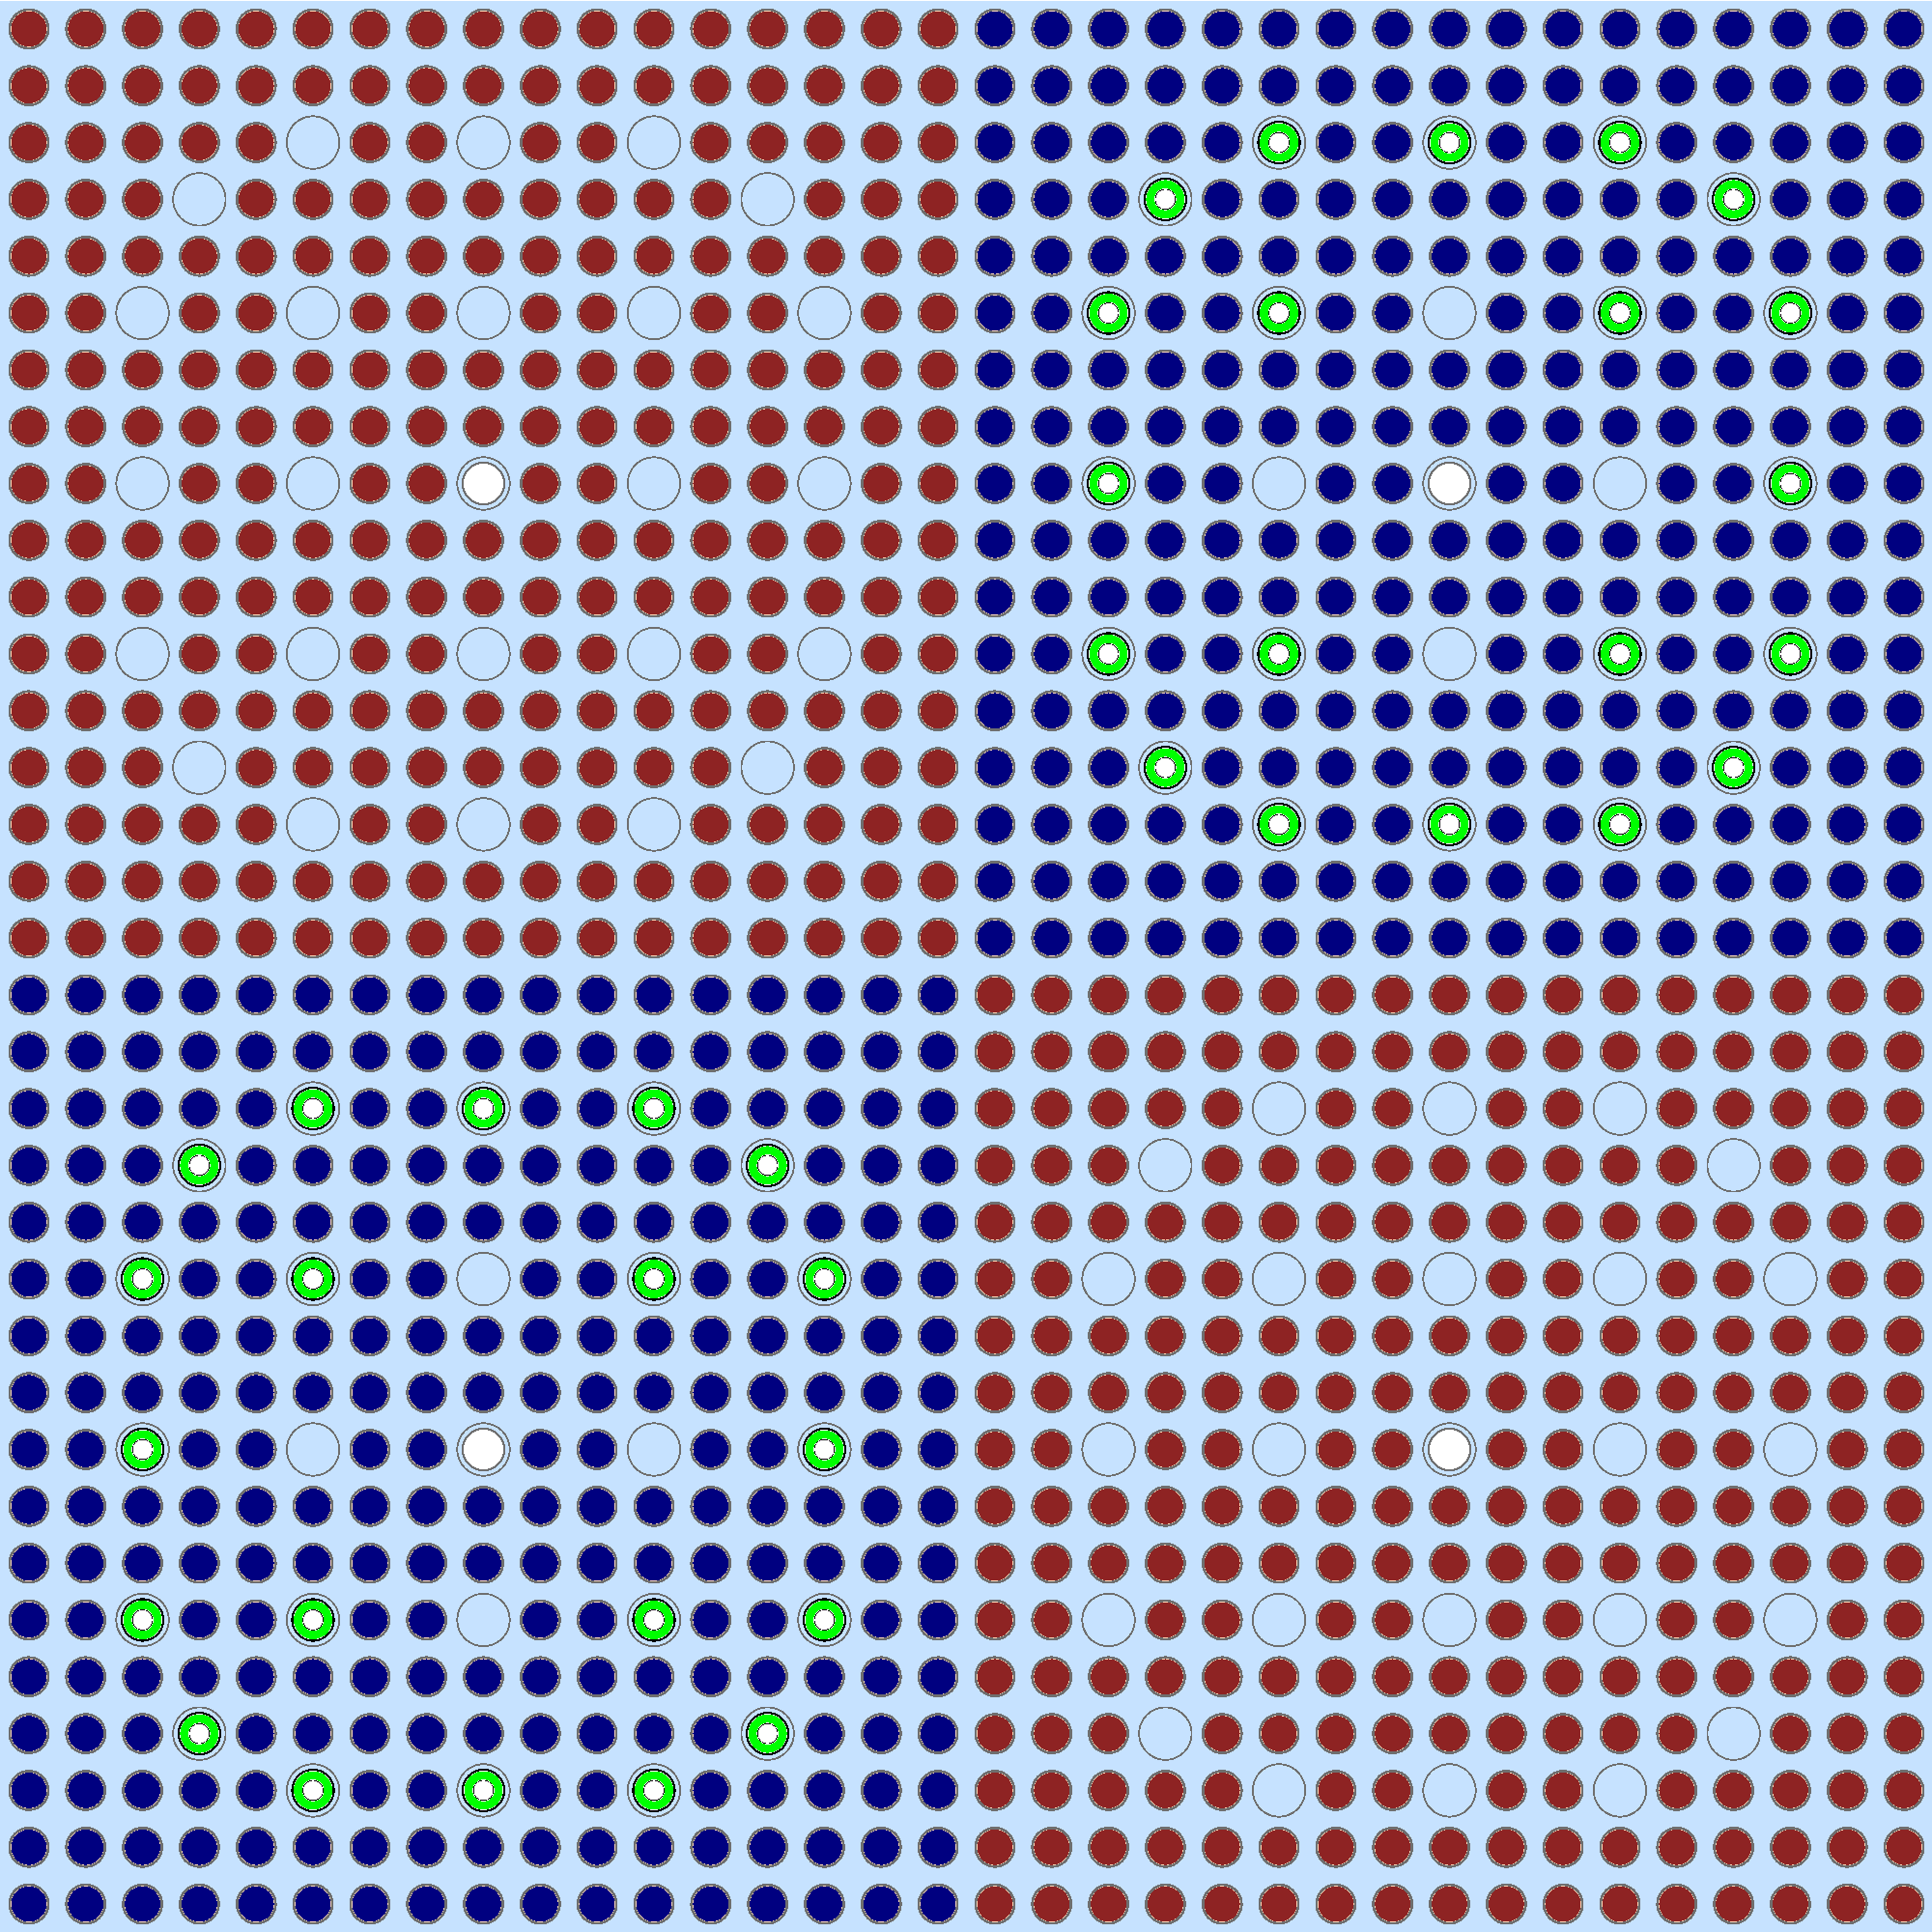
\includegraphics[width=0.9\linewidth]{figures/benchmarks/2x2}
  \caption{}
  \label{fig:2x2}
\end{subfigure}%
\begin{subfigure}{0.47\textwidth}
  \centering
  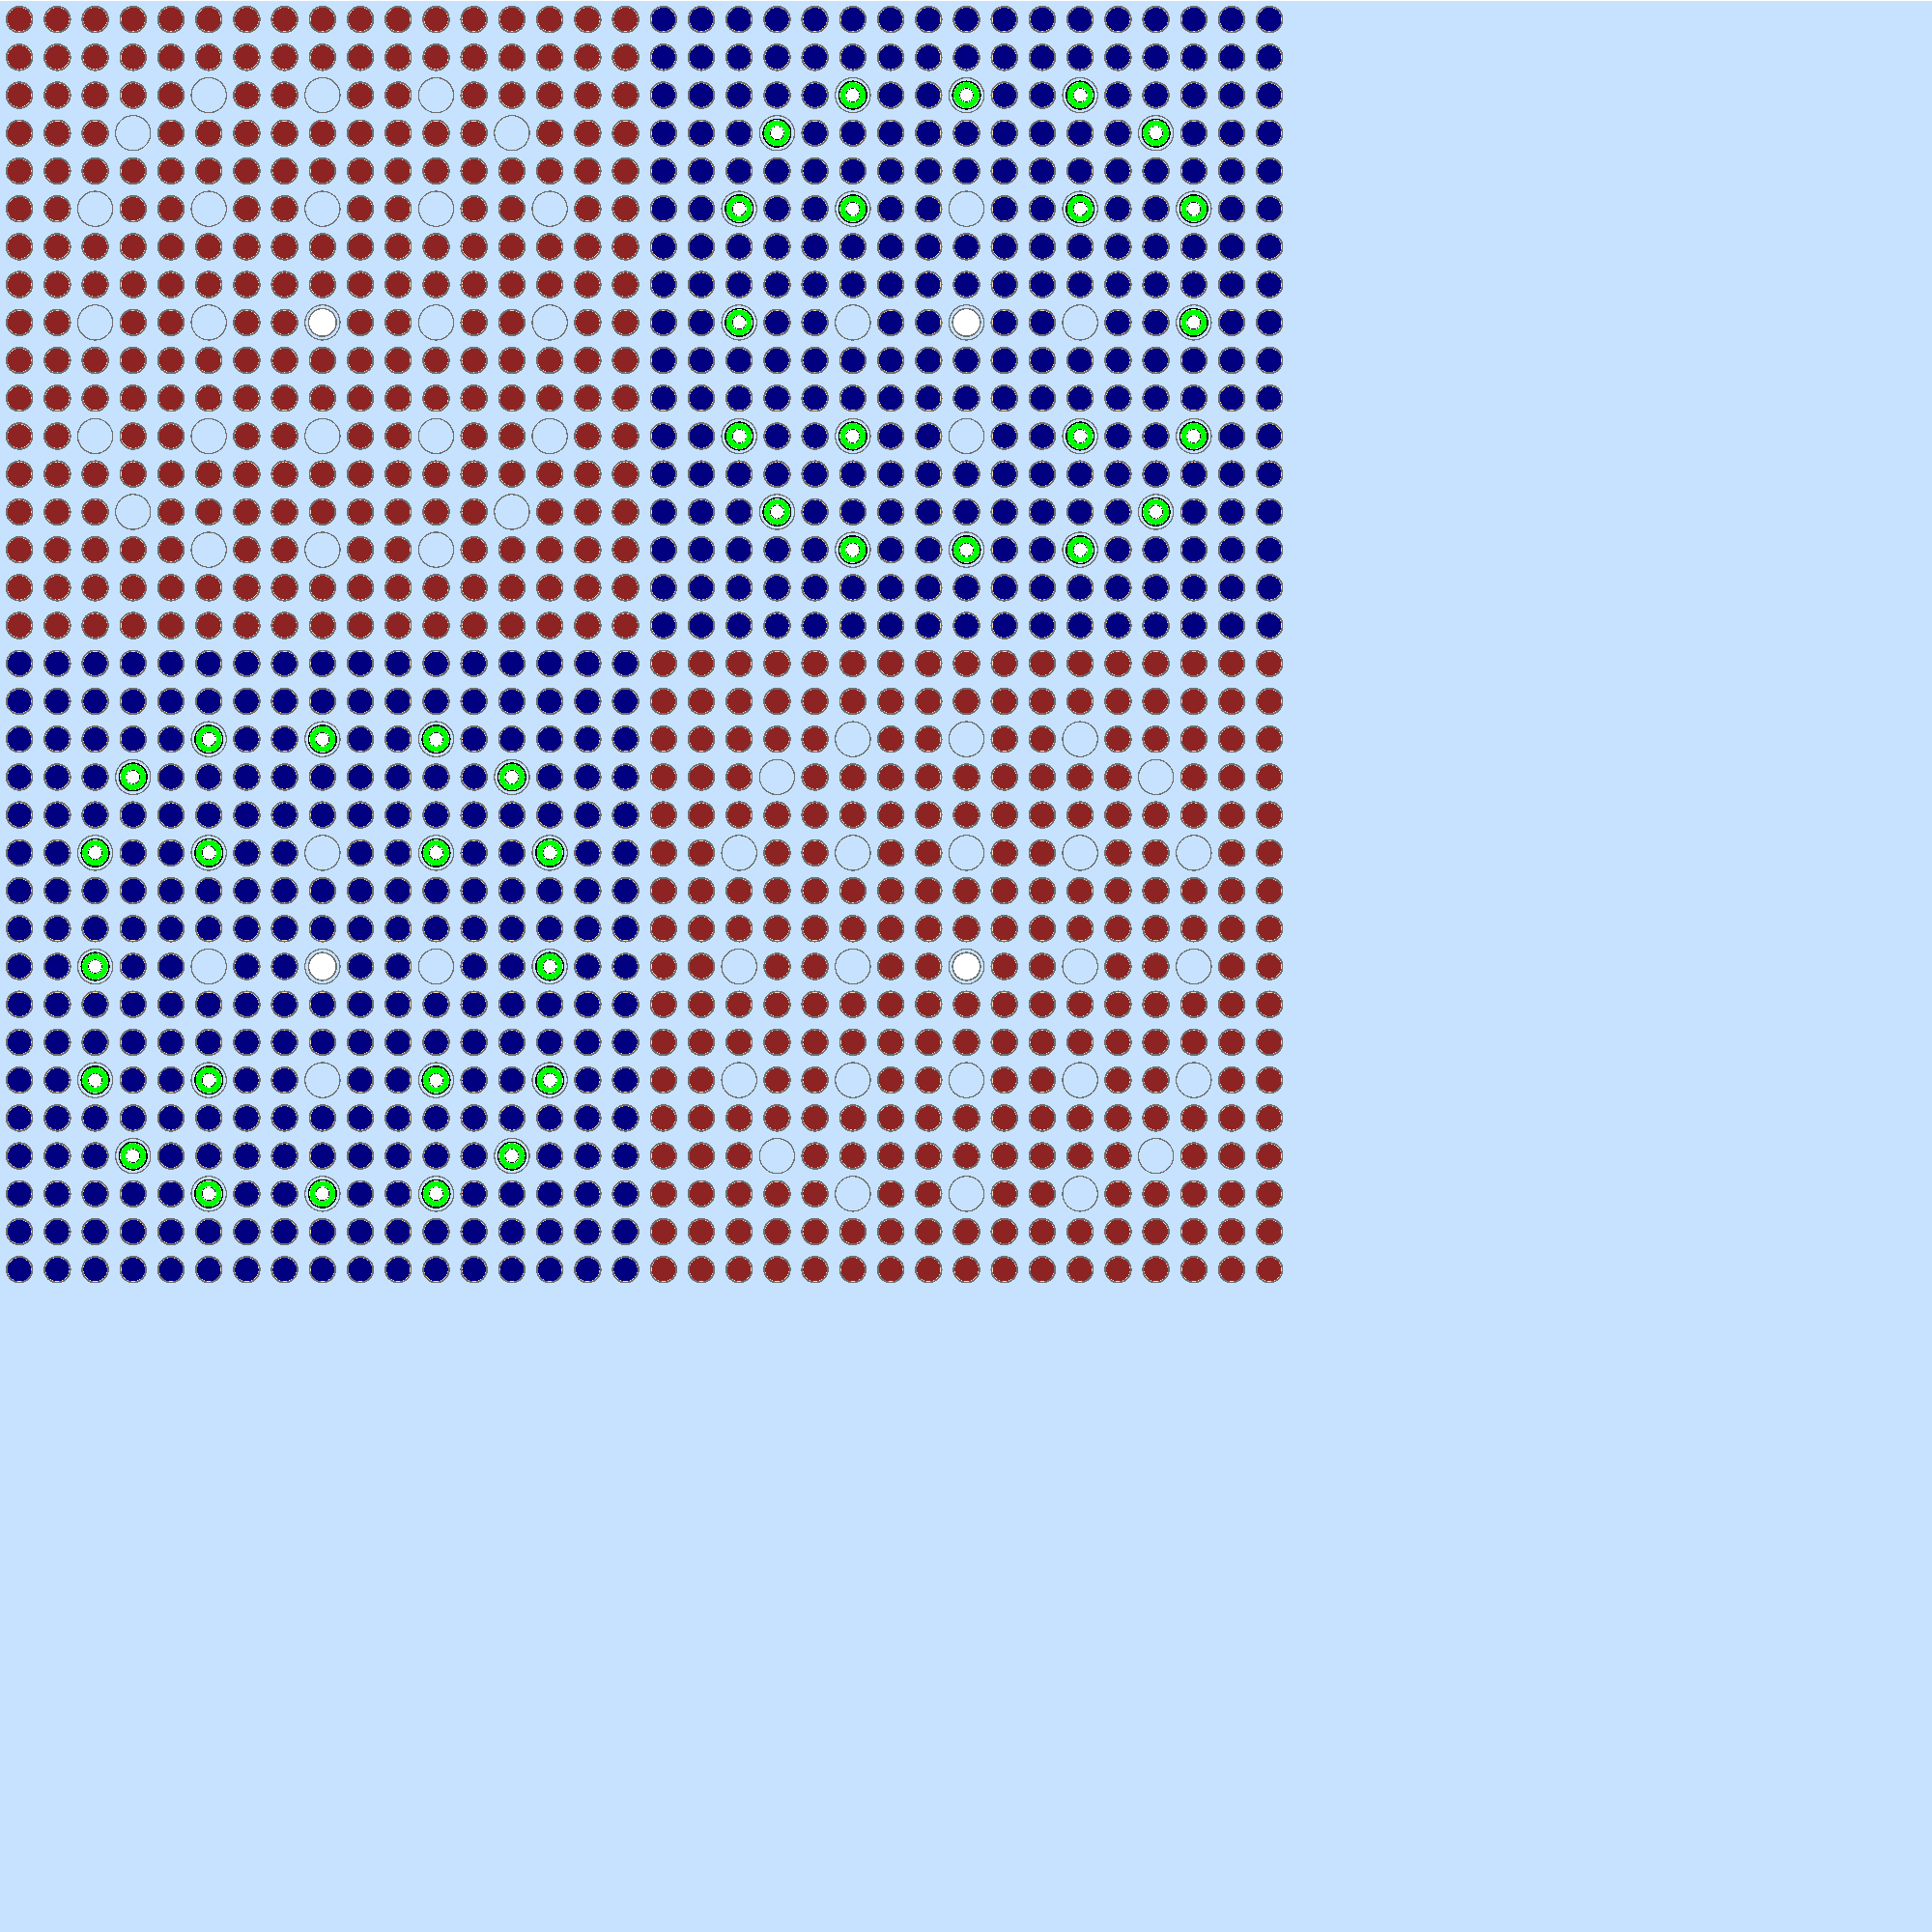
\includegraphics[width=0.9\linewidth]{figures/benchmarks/reflector}
  \caption{}
  \label{fig:reflector}
\end{subfigure}
\caption[A reflected 2$\times$2 colorset]{A 2$\times$2 colorset of BEAVRS assemblies with periodic boundary conditions (a), and the same colorset surrounded by a water reflector with reflective (left and top) and vacuum (right and bottom) boundary conditions (b).}
\label{fig:benchmark-geometries}
\end{figure}

%%%%%%%%%%%%%%%%%%%%%%%%%%%%%%%%%%%%%%%%%%
\subsection*{Validation Metrics}

-eigenvalues \\
-fission rates \\
-U-238 capture rates \\
-only present U-238 capture rates here \\

\clearpage

%%%%%%%%%%%%%%%%%%%%%%%%%%%
\section*{Results}

%%%%%%%%%%%%%%%%%%%%%%%%%%%%%%%%%%%%%%%%%%%%%%%%%
\subsection*{\textit{i}MGXS Clustered Geometries}

\begin{figure}[h!]
\centering
\begin{subfigure}{0.47\textwidth}
  \centering
  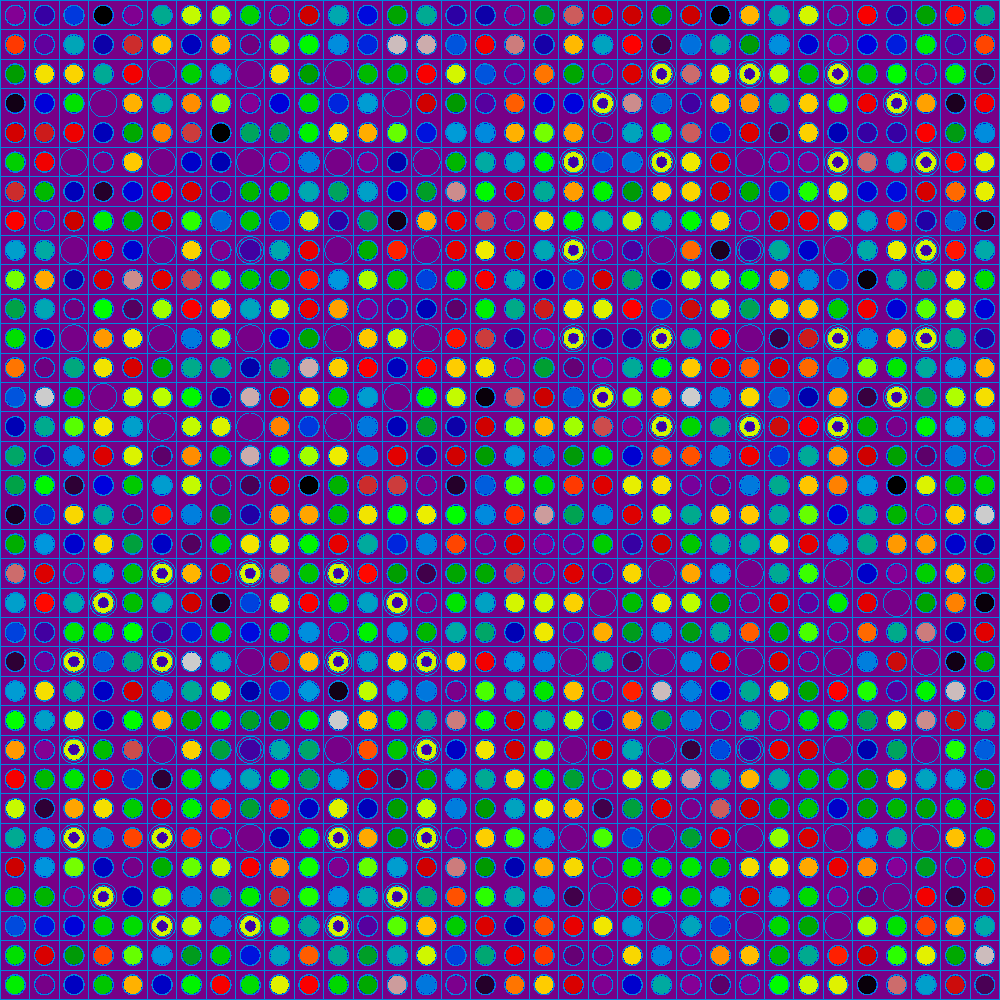
\includegraphics[width=0.7\linewidth]{figures/quantification/homogenization/2x2-degenerate-materials}
  \caption{}
  \label{fig:2x2-degenerate}
\end{subfigure}%
\begin{subfigure}{0.47\textwidth}
  \centering
  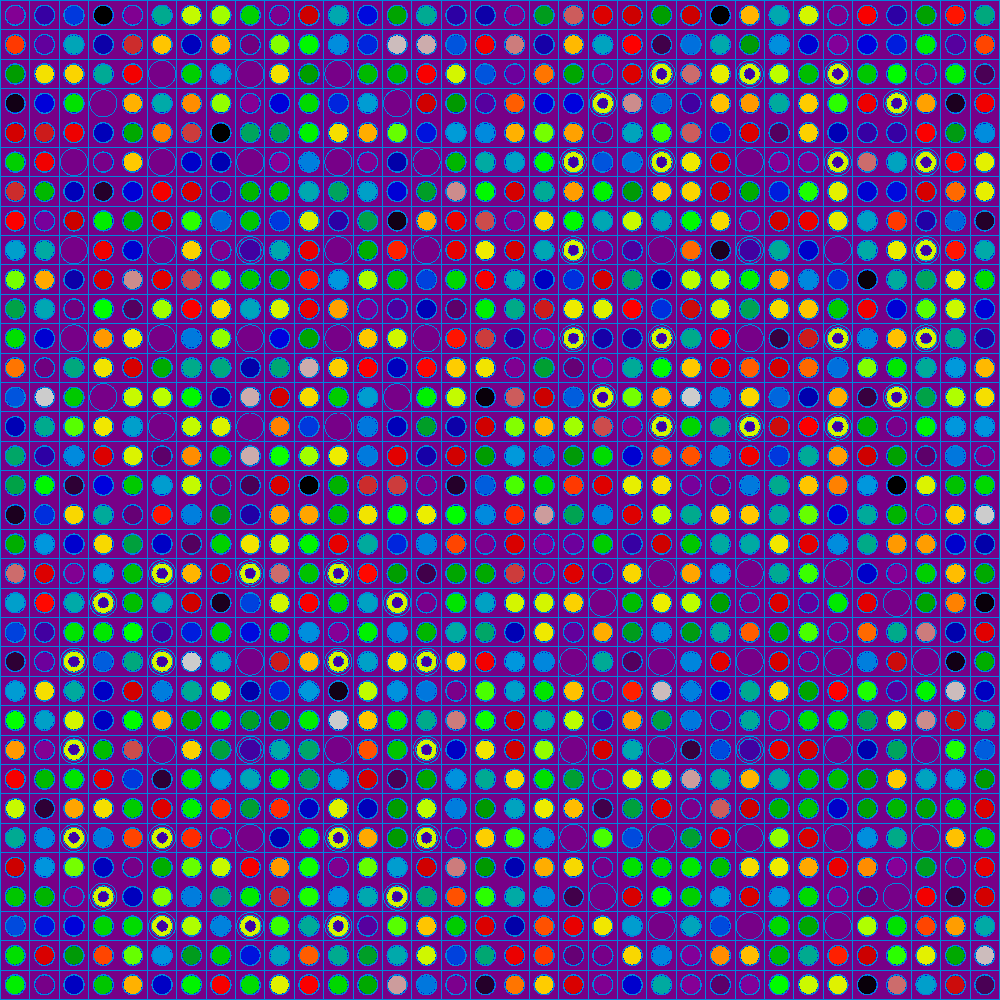
\includegraphics[width=0.7\linewidth]{figures/quantification/homogenization/2x2-degenerate-materials}
  \caption{}
  \label{fig:reflector-degenerate}
\end{subfigure}
\begin{subfigure}{0.47\textwidth}
  \centering
  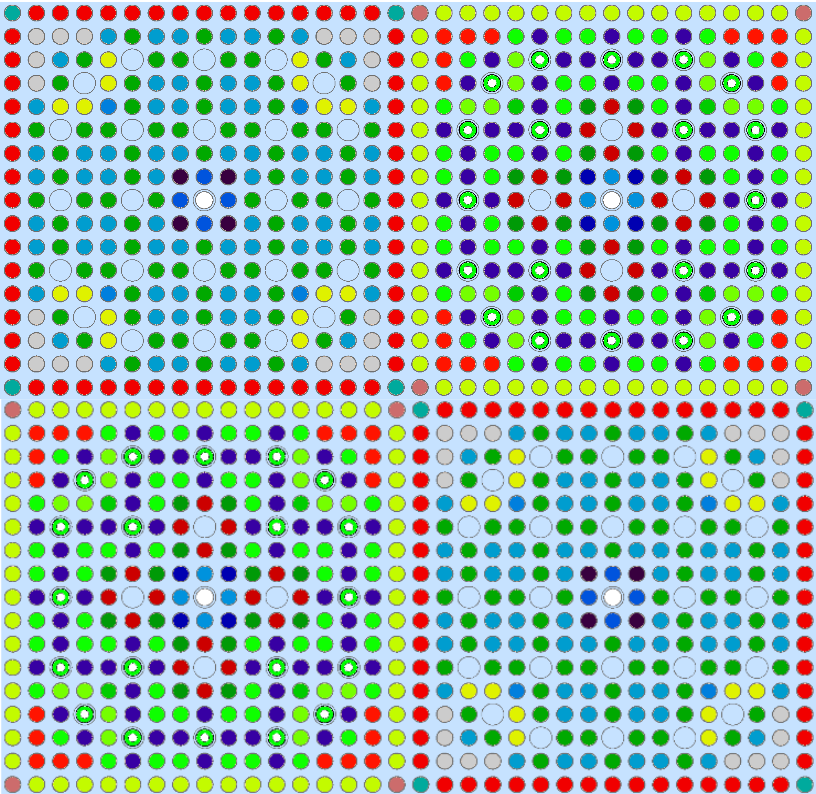
\includegraphics[width=0.7\linewidth]{figures/patterns/lns/2x2/materials}
  \caption{}
  \label{fig:2x2-lns}
\end{subfigure}%
\begin{subfigure}{0.47\textwidth}
  \centering
  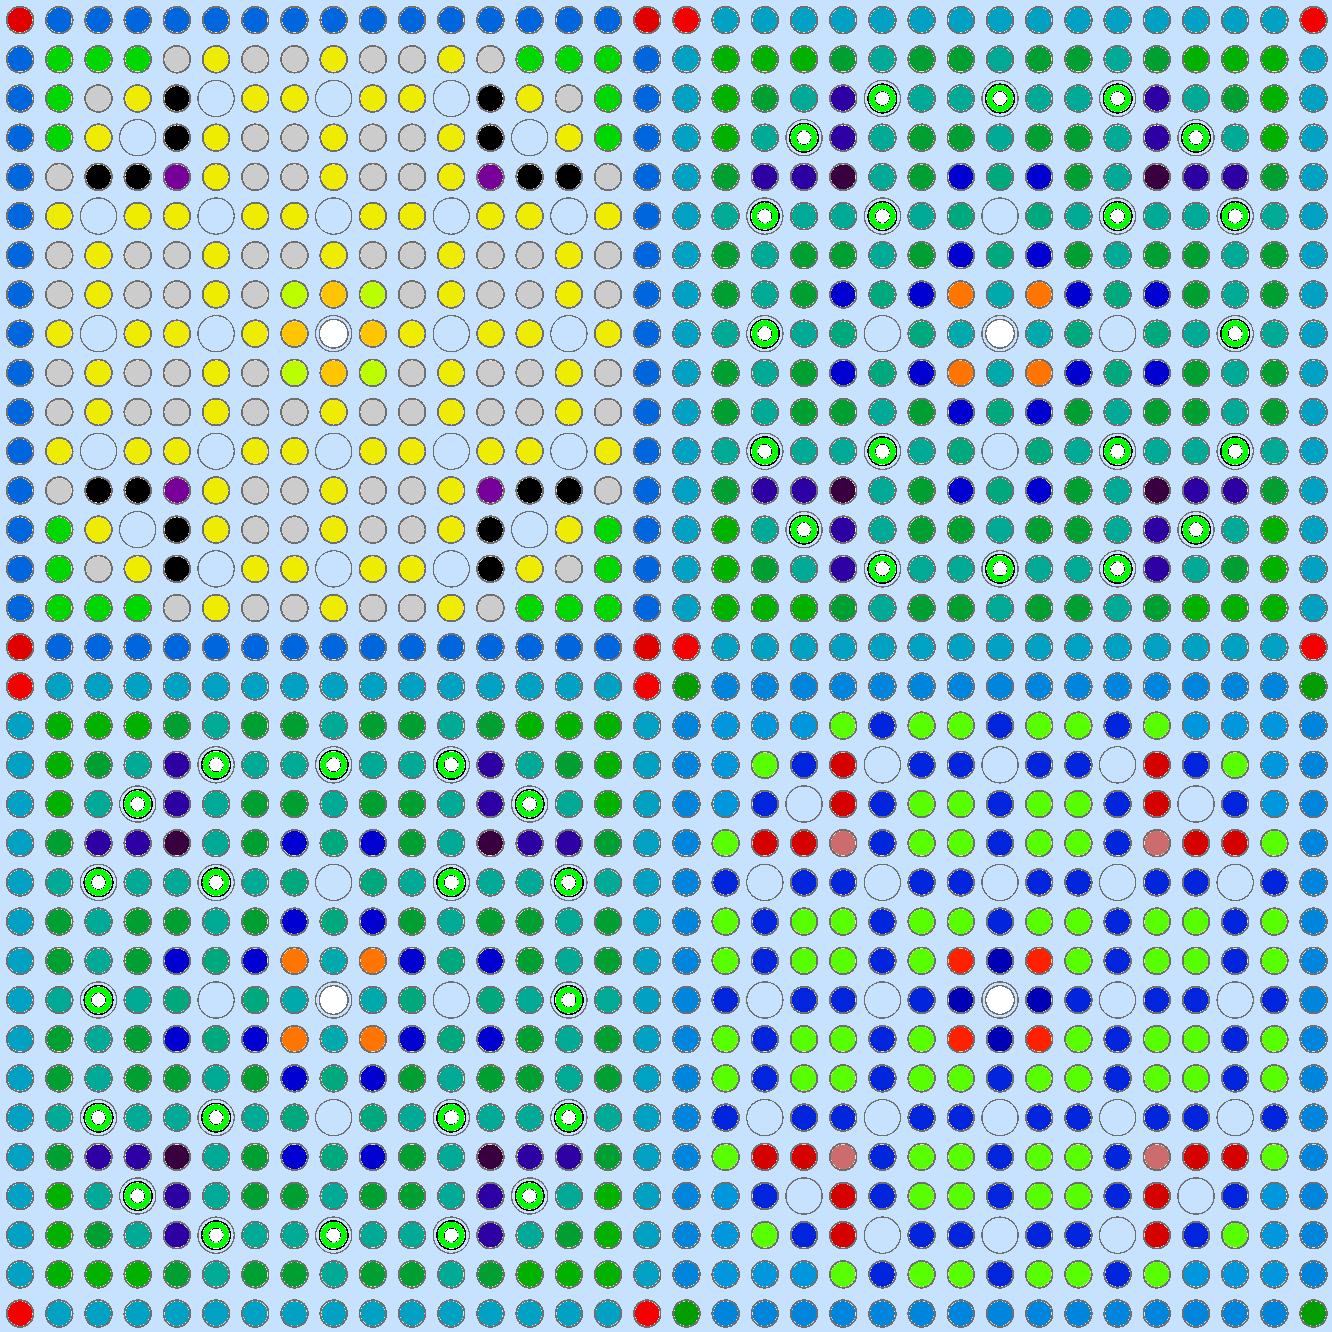
\includegraphics[width=0.7\linewidth]{figures/patterns/lns/reflector/materials}
  \caption{}
  \label{fig:reflector-lns}
\end{subfigure}
\begin{subfigure}{0.47\textwidth}
  \centering
  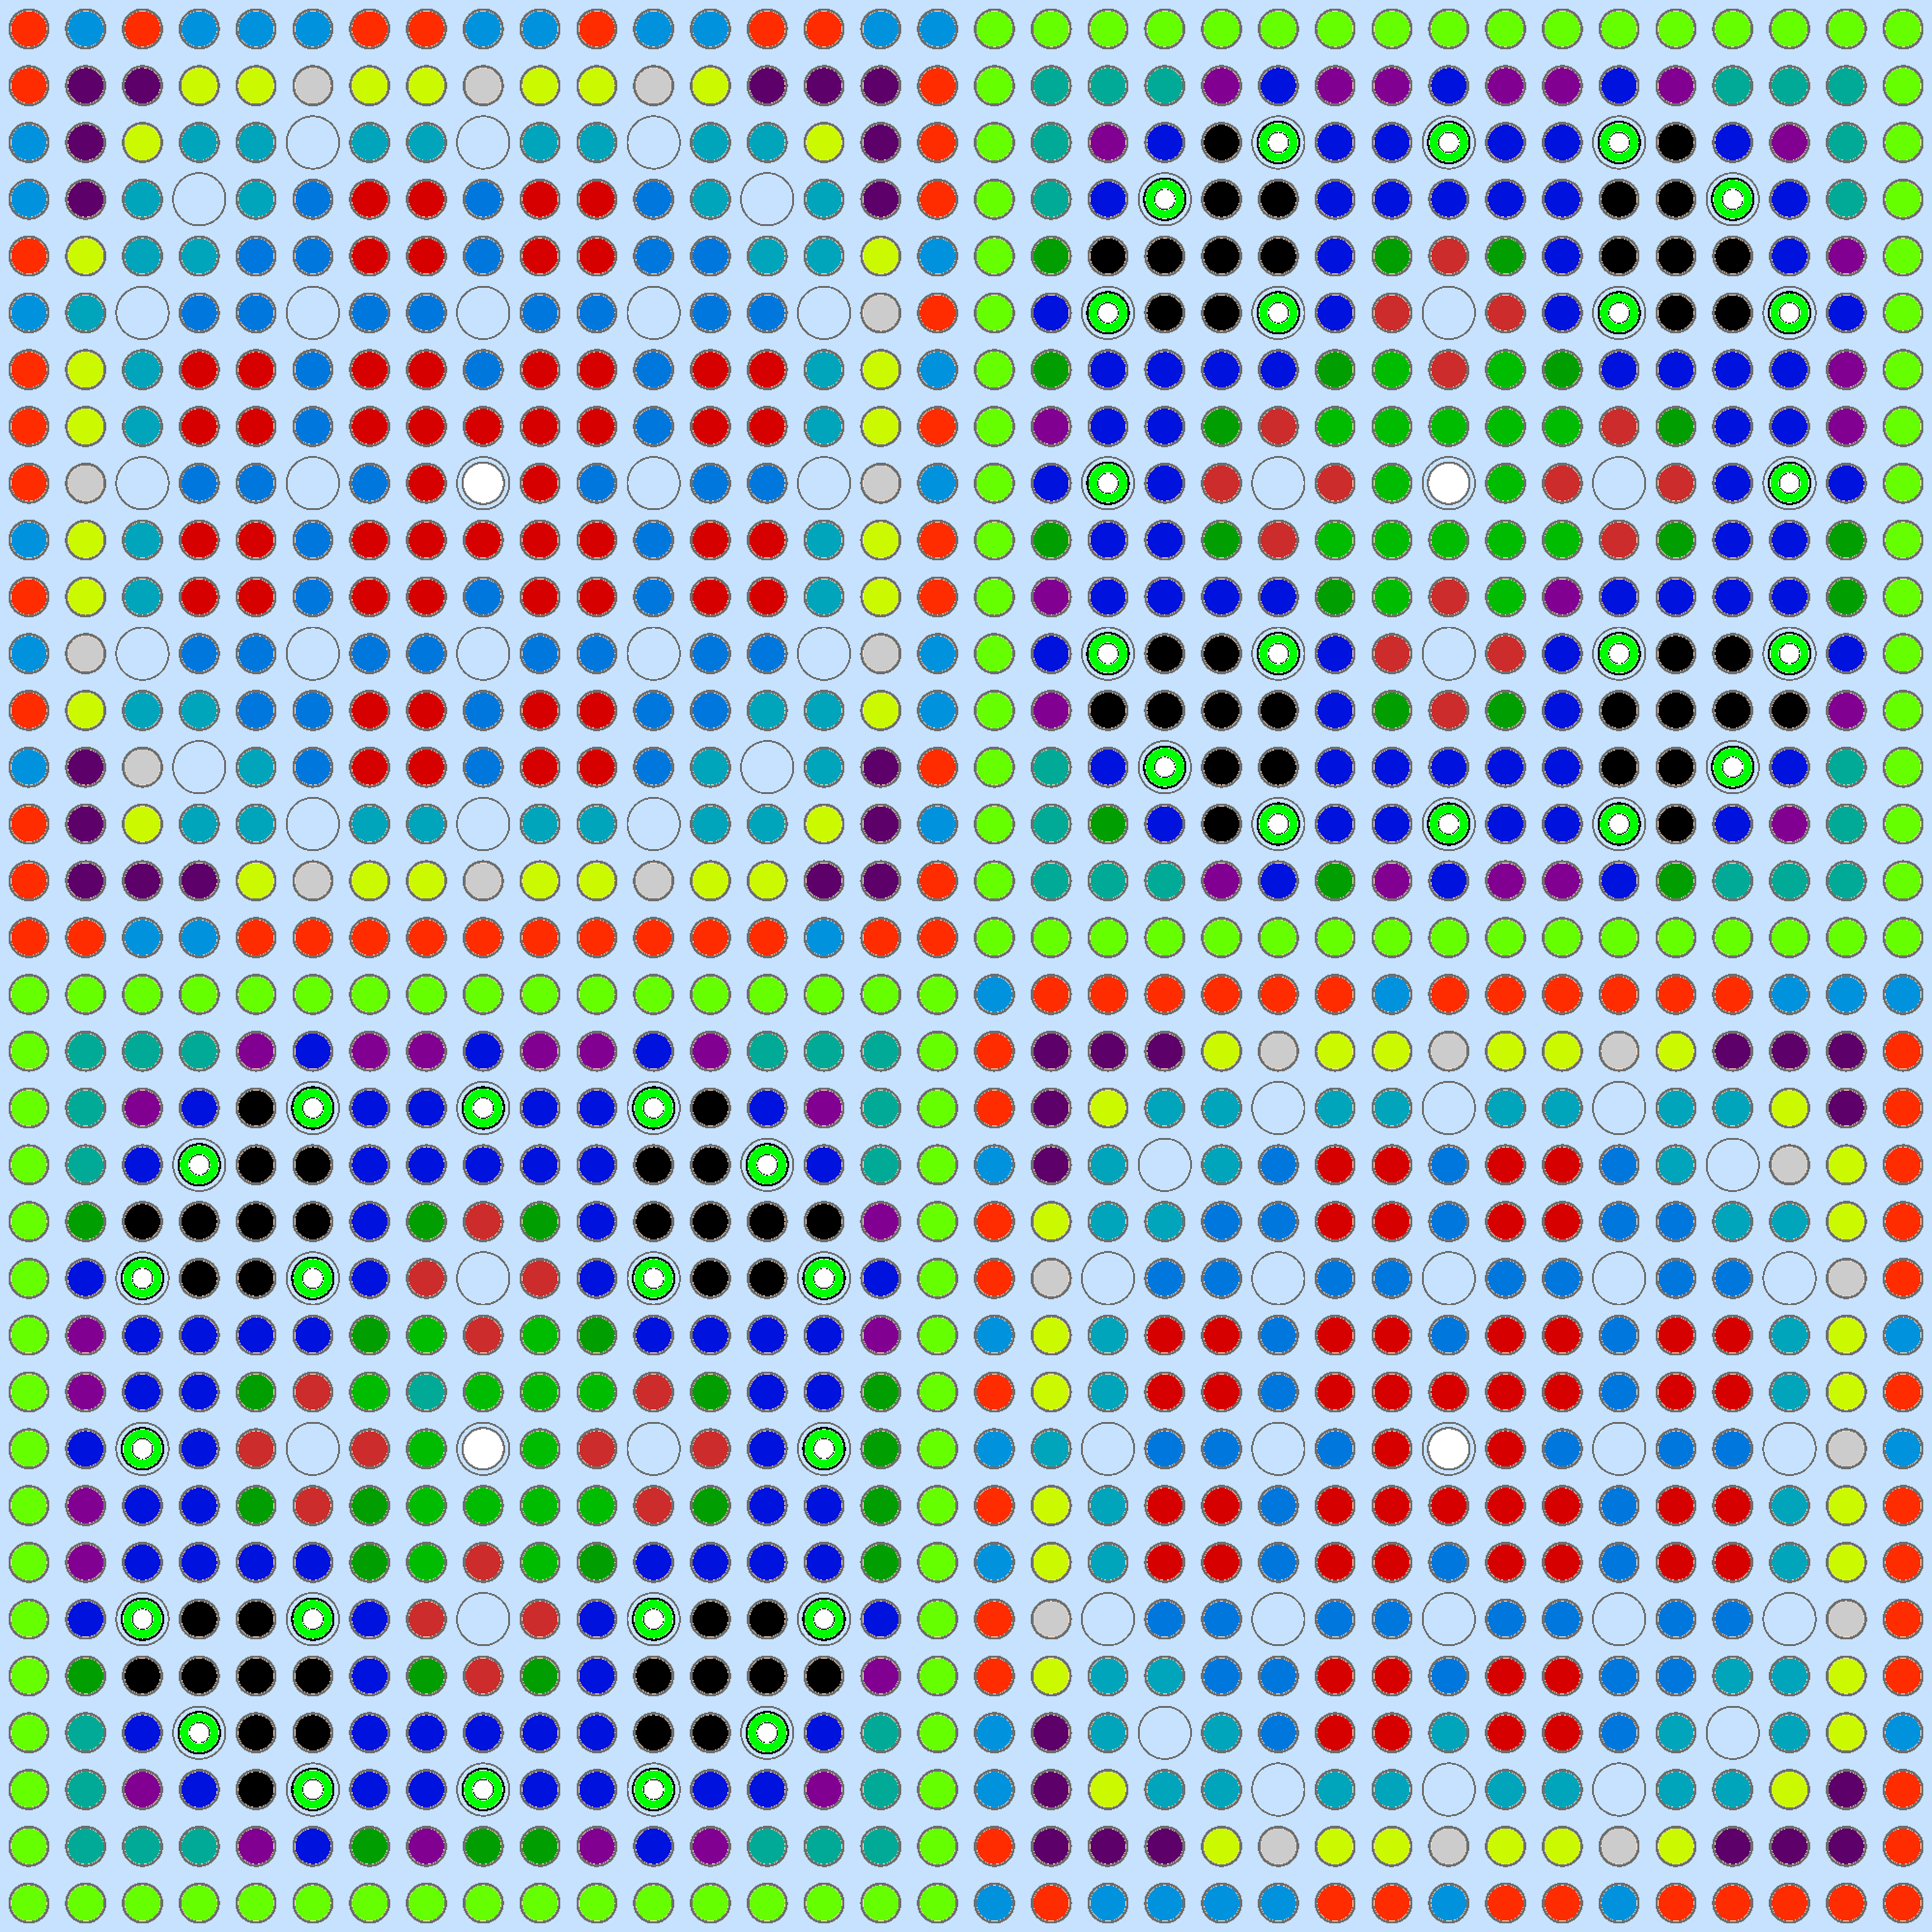
\includegraphics[width=0.7\linewidth]{figures/unsupervised/geometries/with-features/8-clusters/combined/2x2}
  \caption{}
  \label{fig:2x2-8-clusters}
\end{subfigure}%
\begin{subfigure}{0.47\textwidth}
  \centering
  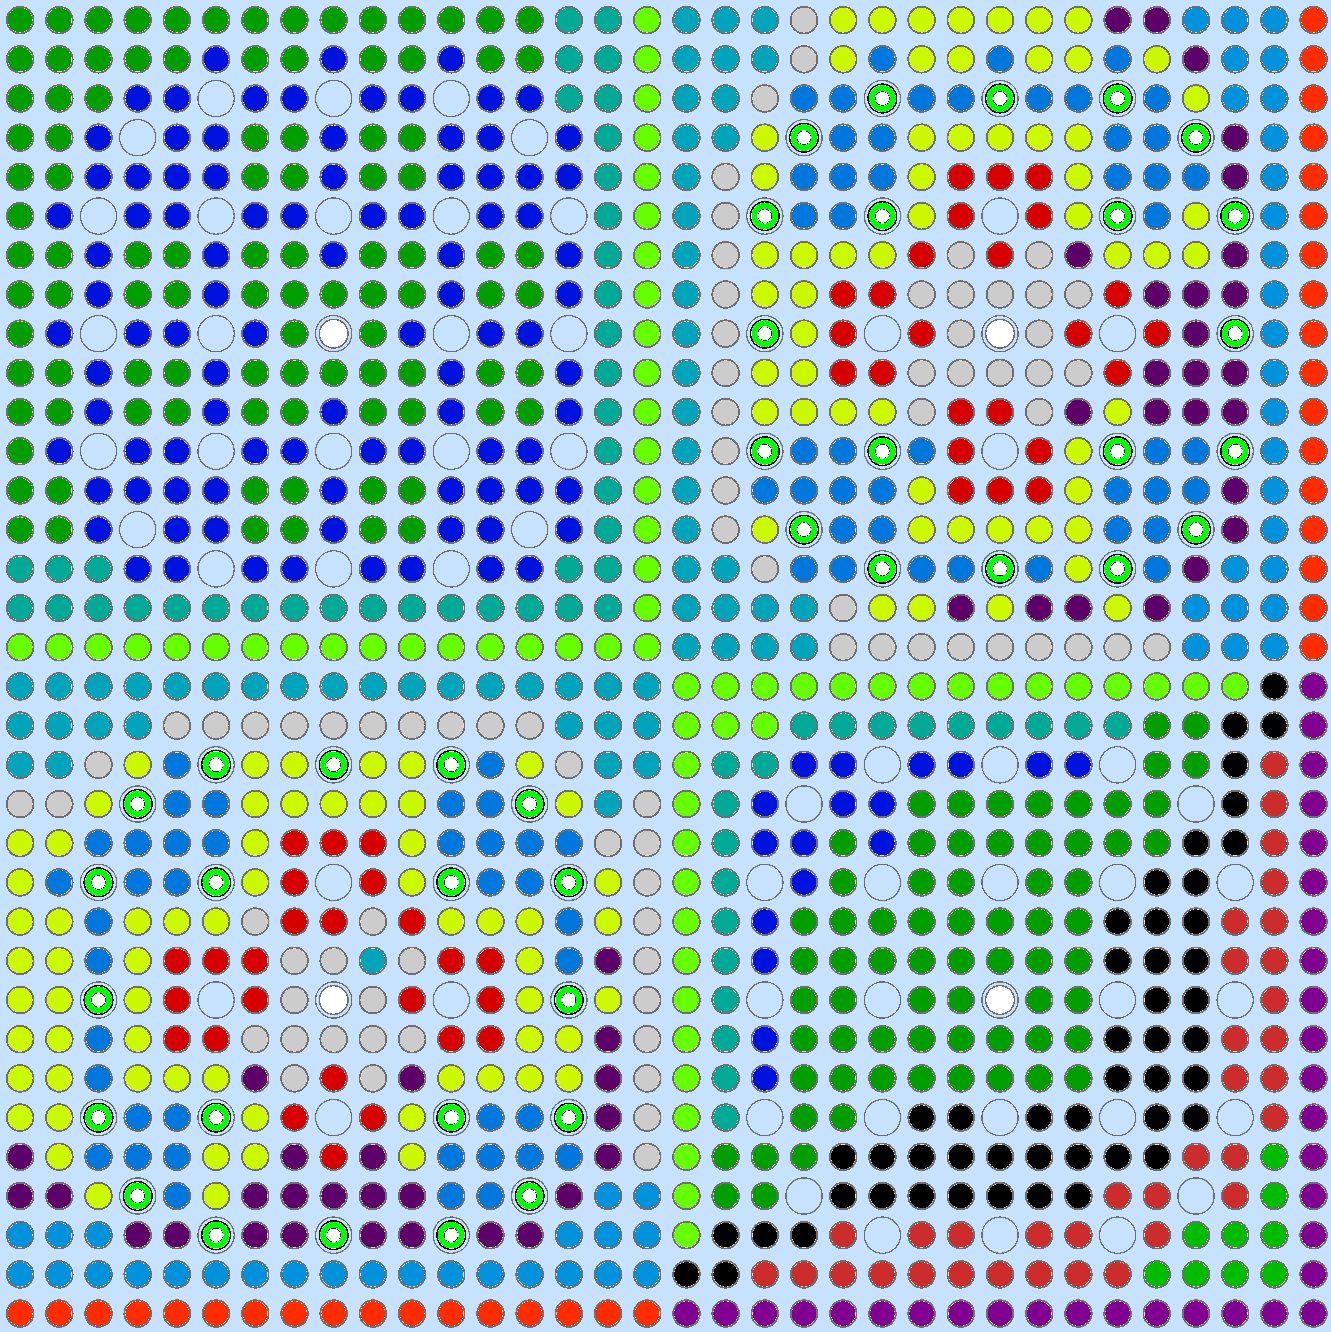
\includegraphics[width=0.7\linewidth]{figures/unsupervised/geometries/with-features/8-clusters/combined/reflector}
  \caption{}
  \label{fig:reflector-8-clusters}
\end{subfigure}
\caption[Materials for the 2$\times$2 colorsets]{The materials for the periodic 2$\times$2 colorset with degenerate, LNS \textit{i}MGXS spatial homogenization are illustrated in (a), (c) and (e), while those for the colorset with a water reflector are depicted in (b), (d) and (f). The materials for the \textit{i}MGXS scheme represent 8 GMM clusters.}
\label{fig:colorset-geometries}
\end{figure}

\clearpage

%%%%%%%%%%%%%%%%%%%%%%%%%%%%%%%%%%%%%%%%%%%%%%%%
\subsection*{Pin-Wise U-238 Capture Rate Errors}

\begin{figure}[h!]
\centering
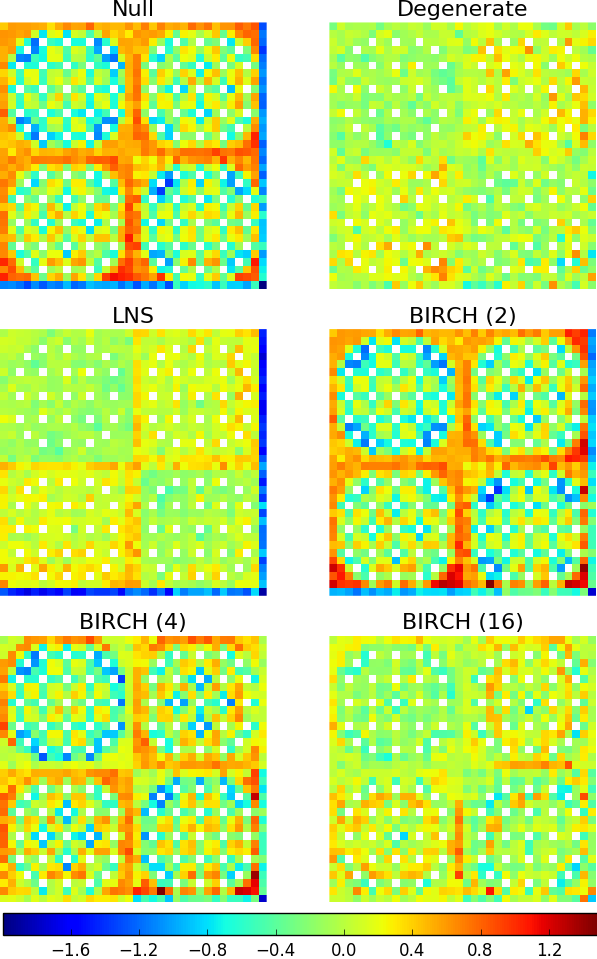
\includegraphics[width=0.8\linewidth]{figures/results/spatial/reflector/capt-err}
\vspace{2mm}
\caption[U-238 capture rate errors for the 2$\times$2 colorset with reflector]{U-238 capture rate percentage relative errors for the 2$\times$2 colorset with a water reflector with null, degenerate, LNS and \textit{i}MGXS spatial homogenization with 2, 8 and 16 GMM clusters.}
\label{fig:refl-capt-err}
\end{figure}

\clearpage

%%%%%%%%%%%%%%%%%%%%%%%%%%%%%%%%%%%%%%%%%%%%%%%%%%%%
\subsection*{Comparing Pin-Wise U-238 Capture Rates}

\begin{figure}[h!]
\centering
\begin{subfigure}{0.9\textwidth}
  \centering
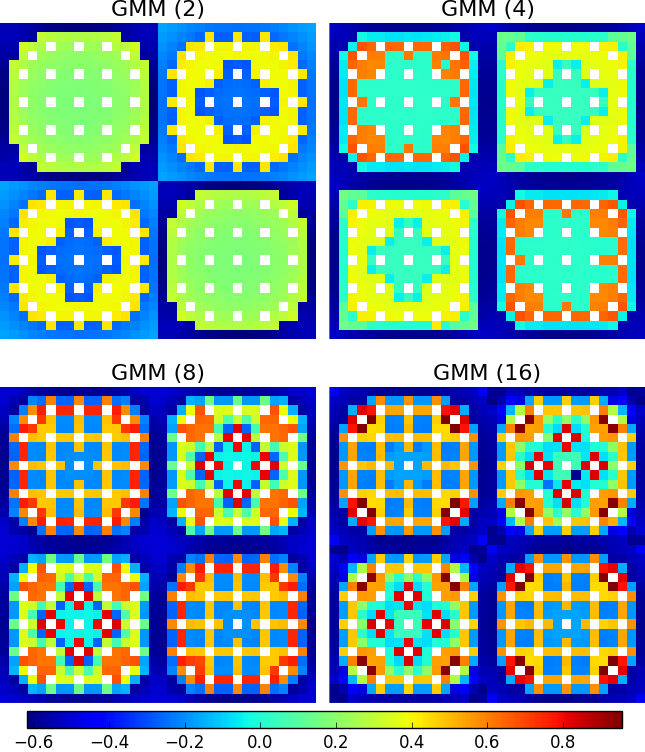
\includegraphics[width=0.55\linewidth]{figures/results/compare/2x2/compare-capt}
  \caption{}
  \label{fig:refl-capt-rates-comp-refl}
\end{subfigure}
\par\bigskip
\begin{subfigure}{0.9\textwidth}
  \centering
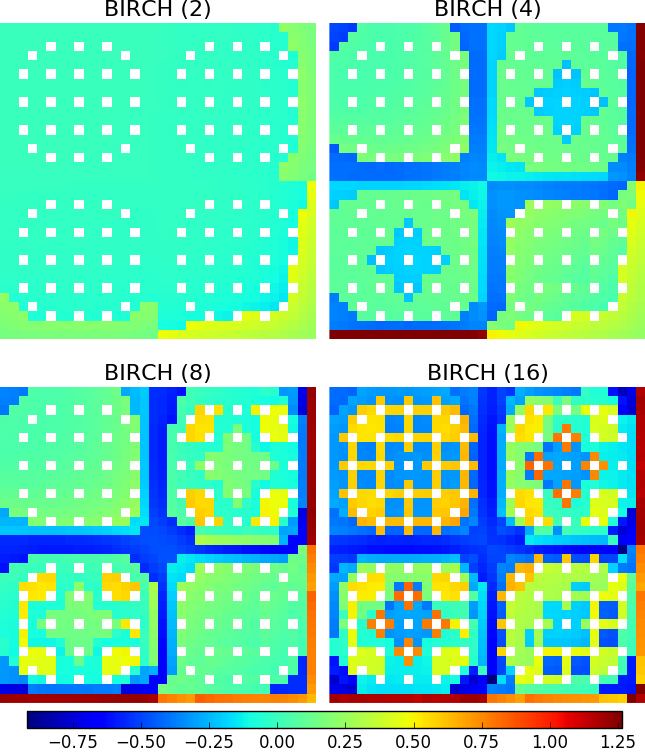
\includegraphics[width=0.55\linewidth]{figures/results/compare/reflector/compare-capt}
  \caption{}
  \label{fig:refl-capt-rates-comp-2x2}
\end{subfigure}
\caption[U-238 capture rate comparison for the colorset]{A comparison of U-238 capture rate spatial distributions for \textit{i}MGXS with GMM clustering and null spatial homogenization schemes for the periodic 2$\times$2 colorset (a) and colorset with a water reflector (b).}
\label{fig:refl-capt-rates-comp}
\end{figure}

\clearpage

%%%%%%%%%%%%%%%%%%%%%%%%%%%%%%%%%%%%%%%%%%%%%%%%
\subsection*{Convergence Rates of MOC Solutions}

\begin{figure}[h!]
\centering
\begin{subfigure}{\textwidth}
  \centering
  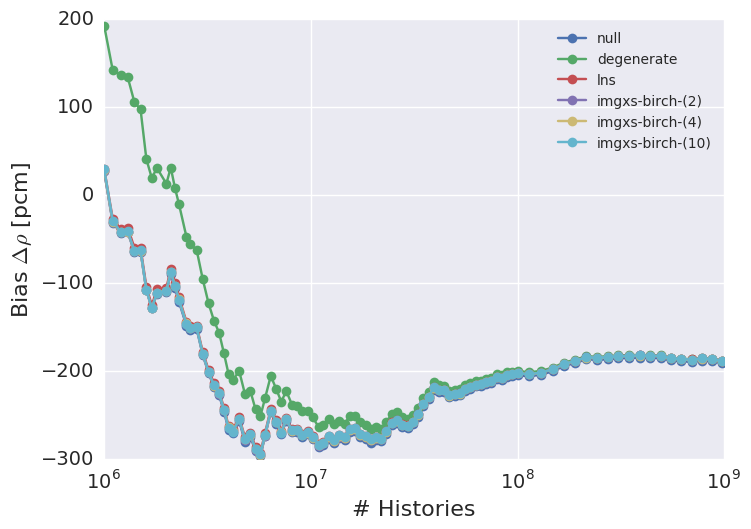
\includegraphics[width=0.8\linewidth]{figures/results/convergence/2x2/keff-bias-evo}
  \caption{}
  \label{fig:2x2-eigenvalue-converge}
\end{subfigure}
\begin{subfigure}{\textwidth}
  \centering
  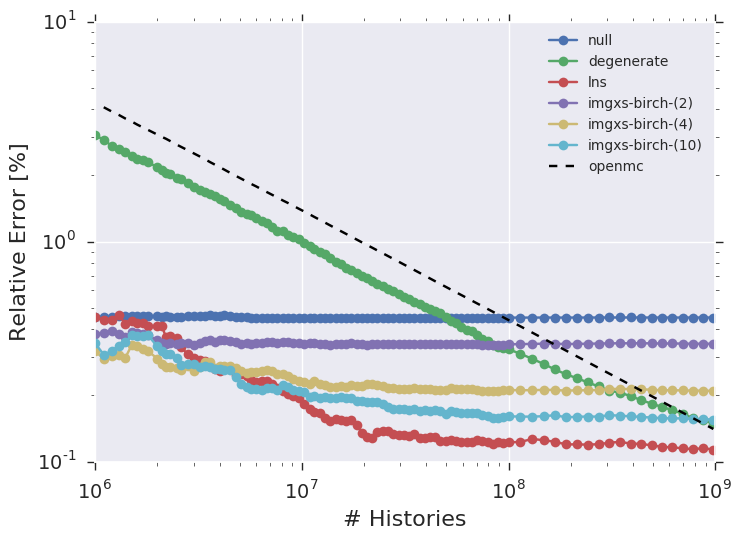
\includegraphics[width=0.8\linewidth]{figures/results/convergence/2x2/mean-capt-err-evo}
  \caption{}
  \label{fig:2x2-capture-converge-mean}
\end{subfigure}
\vspace{2mm}
\caption[Fission rate covergence for the periodic 2$\times$2 colorset]{Convergence of the eigenvalue bias (a) and mean absolute U-238 capture rate percent relative errors (b) for the periodic 2$\times$2 colorset.}
\label{fig:2x2-capture-converge}
\end{figure}

\clearpage

%%%%%%%%%%%%%%%%%%%%%%%%%%%%%%%%%%%%%%%%%%%%%%%%%%%%%%%%%
\subsection*{Runtimes for Spatial Homogenization Schemes}

\begin{table}[ht!]
  \centering
  \caption[Runtimes]{Runtimes.}
  \small
  \label{table:imgxs-runtimes}
  \vspace{6pt}
  \begin{tabular}{l l R{2.5cm} S[table-format=3.2] S[table-format=3.2] S[table-format=3.2]}
  \toprule
  & & & \multicolumn{3}{c}{\bf Runtime [core-hours]} \\
  \cline{4-6}
  \multirow{-2}{*}{\bf Benchmark} &
  \multirow{-2}{*}{\bf Scheme} &
  \multirow{-2}{*}{\bf \# Particles} &
  \multicolumn{1}{c}{\bf OpenMC} &
  \multicolumn{1}{c}{\bf OpenMOC} &
  \multicolumn{1}{c}{\bf Total} \\
  \midrule
\multirow{4}{*}{\parbox{2.5cm}{1.6\% Assm}} & Reference & 550,000,000 & 57.2 & & 57.2 \\
& Null & 100,000 & 0.02 & 0.36 & 0.38 \\
& Degenerate & 115,000,000 & 27.7 & 0.40 & 28.1 \\
& \textit{i}MGXS & 4,000,000 & 0.96 & 0.38 & 1.34 \\
  \midrule
\multirow{4}{*}{\parbox{2.5cm}{3.1\% Assm}} & Reference & 550,000,000 & 50.7 & & 50.7 \\
& Null & 100,000 & 0.02 & 0.40 & 0.42 \\
& Degenerate & 115,000,000 & 25.3 & 0.40 & 25.7 \\
& \textit{i}MGXS & 4,000,000 & 0.88 & 0.37 & 1.25 \\
  \midrule
\multirow{4}{*}{\parbox{2.5cm}{3.1\% Assm w/ 20 BPs}} & Reference & 550,000,000 & 50.1 & & 50.1 \\
& Null & 100,000 & 0.02 & 0.41 & 0.43 \\
& Degenerate & 115,000,000 & 27.7 & 0.41 & 28.1 \\
& \textit{i}MGXS & 4,000,000 & 0.96 & 0.42 & 1.38 \\
  \midrule
\multirow{4}{*}{\parbox{2.5cm}{2$\times$2 Colorset}} & Reference & 8,755,000 & 81.7 & & 81.7 \\
& Null & 100,000 & 0.04 & 2.00 & 2.03 \\
& Degenerate & 700,000,000 & 248 & 2.29 & 250 \\
& \textit{i}MGXS & 10,000,000 & 3.54 & 1.96 & 5.50 \\
  \midrule
\multirow{4}{*}{\parbox{2.5cm}{2$\times$2 Colorset w/ Reflector}} & Reference & & & & \\
& Null & & & 5.07 & \\
& Degenerate & & & 5.36 & \\
& \textit{i}MGXS & & & 4.90 & \\
  \midrule
\multirow{4}{*}{\parbox{2.5cm}{BEAVRS Quarter Core}} & Reference & & & & \\
& Null & & & 419 & \\
& Degenerate & & & 426 & \\
& \textit{i}MGXS & & & 423 & \\
  \bottomrule
\end{tabular}
\end{table}

\clearpage

%%%%%%%%%%%%%%%%%%%%%%%%%%%%%%%%%%%%%%%%%%%%%%%%%%%%%%%%%%%%%%%%%%%%%%%%%%%%%%%%
\section*{Conclusions}

%%%%%%%%%%%%%%%%%%%%%%%%%%%%%%%%%%%%%%%%
\subsection*{Contributions to the Field}

-tightly coupled framework for MC and MOC for MGXS \\
-useful for both MGXS generation as well as validation of MOC \\
-identified fundamental issue with flux separability approx. and 

%%%%%%%%%%%%%%%%%%%%%%%%%
\subsection*{Future Work}

-speed up OpenMOC full core: \\
  -find a way use quarter assembly CMFD mesh \\
  -linear source to reduce number of spatial zones \\
  -vectorize transport solver over energy groups \\

\break

evaluate \textit{i}MGXS scheme:
-add anisotropic scattering to OpenMOC to enable solution of the ``correct'' problem
-systematic study of featues -- ones actually matter? \\
-systematic study to understand impact of dimensionality reduction \\
-systematic study to understand impact of clustering algorithms \\
-more research into model selection schemes -- none of them robustly works for my case studies! \\
-evaluate \textit{i}MGXS with clustering ``on-the-fly'' with noisy MC tally data \\
-can \textit{i}MGXS reduce the number of necessary energy groups?? \\

\break

reach goals:\\
-multi-physics applications: moderator density, fuel temperature, burnup, etc. as features \\
-machine learning to optimize energy group structures \\


%%%%%%%%%%%%%%%%%%%%%%%%%%%%%%%%%%%%%%%%%%%%%%%%%%%%%%%%%%%%%%%%%%%%%%%%%%%%%%%%
%%%%%%%%%%%%%%%%%%%%%%%%%%%%%%%%%%%%%%%%%%%%%%%%%%%%%%%%%%%%%%%%%%%%%%%%%%%%%%%%
% BIBLIOGRAPHY

\begin{singlespace}
\bibliographystyle{ans}
\bibliography{references}
\end{singlespace}

\end{document}
